% !TEX program = xelatex
\documentclass[twocolumn,superscriptaddress,english,showpacs,longbibliography]{revtex4-2}
\usepackage[colorlinks=true,urlcolor=blue,citecolor=blue,linkcolor=blue]{hyperref} 

\usepackage{svg}
\usepackage{amsmath}
\usepackage{graphicx}% Include figure files
\usepackage{textcomp}
\usepackage{bm}% bold math
\usepackage{color}
\usepackage{amssymb}
\usepackage{amsthm}
\usepackage{graphicx}
\usepackage{color}
\usepackage{mathrsfs}
\usepackage{float}
\usepackage{indentfirst}
\usepackage{txfonts}
\usepackage{algorithm}  
\usepackage{algpseudocode}  
\usepackage{balance}
\usepackage{flushend}
\usepackage{cleveref}
\usepackage{kbordermatrix}
\usepackage{blkarray}
\usepackage{tikz}
\renewcommand{\algorithmicrequire}{\textbf{Input:}}  % Use Input in the format of Algorithm  
\renewcommand{\algorithmicensure}{\textbf{Output:}} % Use Output in the format of Algorithm  
\newtheorem{hyp}{Hypothesis}

\newcommand{\jinguo}[1]{[{\color{blue}{JGL: #1}}]}
\newcommand{\ym}[1]{[{\color{red}{YM: #1}}]}
\newcommand{\s}{\mathbf {s}}
\newcommand{\net}[1]{{\textsc{#1}}}
\newcommand{\vs}{{\mathbf{s}}}
\newcommand{\vn}{{\mathbf{n}}}
\newcommand{\argmin}{\mathop{\mathrm{argmin}}\limits}
\newcommand{\Eq}[1]{Eq.~(\ref{#1})}
\newcommand{\Fig}[1]{Fig.~\ref{#1}}

\begin{document}

\title{Crystal as a thermodynamic computer}

\author{Authors}
\email{xxx@xxx.com}
\affiliation{
    XXX
}

\begin{abstract}
    Thermodynamic computers are believed to be more energy efficient than conventional computers, however, a practical implementation of a thermodynamic computer is still challenging. In this paper, we propose a thermodynamics driven computer that enables use to perform computation by editing its surface.
    The crystalline structure is based on a universal elementary CA, and is translational invariant in all spacial dimensions. The translational invariance not only makes the crystal easier to be constructed in nature, but also enables the study of the scaling behavior the thermalization process.
    Efficiency of the computation of the proposed thermodynamic computer is demonstrated by numerical results.
\end{abstract}

\maketitle

\section{Introduction}

\jinguo{}
\ym{Need to add a brief summary about the state-of-the-art TCs. Following is some basic summaries of references
\begin{enumerate}
    \item Discussed the architecture of future thermodynamic computer and brought up an idea about the understanding of using TC to solve problems~\cite{hylton2021vision}.
    \item TODO: search for gadgets for array multiplier.
\end{enumerate}
}

Improving the energy efficiency of computation is a major challenge in the development of future computing systems.
The thermodynamic computer (TC)~\cite{conte2019thermodynamic, hylton2021vision} is a new type of computer that uses thermodynamics to perform computation.
Instead of performing the computation deterministically, TCs are stochastic and are driven by thermodynamics.
Physical implementations of TCs include DNA machines~\cite{tanaka2005design} and Ising machines~\cite{gu2012encoding, lucas2014ising, mohseni2022ising, fabre2014optical}.
% memristors~\cite{yang2013memristive, wang2017memristors, kumar2017chaotic, wang2018fully}, 

The computational process of TCs utilizes the tendency of a physical system to evolve towards the state with the lowest free energy.
By manipulating the minimum free energy state of the system, the computation can be performed.
The change of free energy minimum state can be achieved by changing the distribution of the particles in the system, such as in the case of DNA machines~\cite{Feynman2018} or lowering the temperature of the system, such as in the case of Ising machines~\cite{boixo2013experimental}.
The former is known as the Brownian machine, which evolves the system toward the direction of the entropy increase, while the latter are energy based, which evolves the system toward the direction of the energy decrease.

Energy based models are probability one of the most powerful models for computation.
The Ising model is not only capable of universal computation~\cite{gu2012encoding}, and it can be used to formulate many NP problems~\cite{lucas2014ising,mohseni2022ising}.

However, they are notoriously hard to thermalize, even with the help of quantum entanglement~\cite{boixo2013experimental, boixo2014evidence, Pichler2018, Ebadi2022, Nguyen2023}.
There is no evidence yet that they can significantly outperform existing algorithms run on classical computers~\cite{}.
Even when the encoded problem is an easy one, it is not guaranteed that the system can thermalize in polynomial time as we will show in the main text.

Intrigued by the question of how to thermalize and lower the energy of an Ising machine, we propose a new type of TC that has a crystalline structure.
The crystalline structure is based on a universal elementary CA, and is translational invariant in all spacial dimensions.
The translational invariance not only makes the crystal easier to be constructed in nature, but also enables the study of the scaling behavior the thermalization process.
In the rest of this paper, we first show that the crystalline structure can be programmed on its surfaces to perform universal computation \Cref{sec:Overview-of-main-results}.
Then we use numerical results in \Cref{sec:numerical-result} to show that if we thermalize the crystal from the so-called ``deterministic direction'', the crystal can thermalize in time almost linear to the size of the crystal, i.e. efficient computation can be performed.

% The way to lower the free energy is inspired by the process of crystalization.
% The material is orderly grown by slowly moving the temperature gradient in-plane~\cite{Zhang2014}.
% Growing a perfect crystal itself is a computation process of copying the information from one surface to another.
%In the DNA based TC, the DNA enzyme is driven by thermodynamics, and the computation is performed by the enzyme as it moves along the DNA strand. It is a Brownian type computational model~\cite{Feynman2018} that driven by the change of entropy.

% TCs are distinguished by their ability to employ the underlying physics of the computing substrate to accomplish a task.
% For example, TCs may employ naturally occurring device-level fluctuations to explore a state space and to stabilize on low-energy representations, which may then be employed in an engineered task.
% TCs are directly connected to real-world potentials, which drive the evolution of their internal organization.
% A user might program constraints that describe an optimization objective over the external potentials and that capture the TC’s natural tendency to maximize entropy production in the environment while minimizing entropy production internally.
% TCs have the potential to be more energy efficient than conventional computers, and they may be able to solve problems that are difficult for conventional computers to solve.
% TCs are still in the early stages of development, but they have the potential to revolutionize computing in the future.

% A thermodynamic computer is a complex system, driven by thermodynamics when exposed to external potentials. Like quantum computers, TCs are distinguished by their ability
% to employ the underlying physics of computing substrate to
% accomplish a task. For example, TCs may employ naturally
% occurring device-level fluctuations to explore a state space
% and to stabilize on low-energy representations, which may
% then be employed in an engineered task~\cite{conte2019thermodynamic}.

% Comparing with all conventional computers fully controlled by humans, the TC, on the other hand, are directly connected to real-world potentials, which drive the
% evolution of its internal organization. As an example of using a TC, a user might program
% constraints that describe an optimization objective
% over the external potentials and that capture the TC’s
% natural tendency to maximize entropy production in the
% environment while minimizing entropy production internally~\cite{conte2019thermodynamic}.

%Quantum annealing outperform classical annealing~\cite{boixo2013experimental, boixo2014evidence}.
%Firstly introduced Rydberg atoms to solve MIS problem with quantum property~\cite{Pichler2018}. Utilized quantum annealing on Rydberg arrays to efficiently solve the combinatorial optimization problem~\cite{Nguyen2023}

%Provided basic knowledge about computational model like DNA Enzyme driven by thermodynamics, raised concepts of reversible computing and gradient power~\cite{Feynman2018}.

%Proved Ising model is capable of universal computation~\cite{gu2012encoding}. Provided Ising formulations of many NP problems~\cite{lucas2014ising}.
%Reviewed various type of Ising machines as hardware analog solvers of combinatorial optimization problems~\cite{mohseni2022ising}.
%A special optical form Ising machine~\cite{fabre2014optical}.
%Other type of TCs like memristors~\cite{yang2013memristive, wang2017memristors, kumar2017chaotic,wang2018fully}, DNA machine~\cite{tanaka2005design}. 




\section{Overview of the computation model}\label{sec:Overview-of-main-results}
The TC we are proposing is shown in \Cref{Surface-programmable-thermodynamic computer}. It features a crystalline structure that encodes the time evolution of a universal CA that capable of performing universal computation.
To encode a $d$-dimensional CA, we need a $d+1$-dimensional crystal. The extra dimension is used to encode the time-axis of the CA.
For simplicity, we will focus on the one dimensional 110 rule elementary CA in the rest of this paper.
The physical implementation of the TC is based on the Ising model, where we use the spin up and down to encode the state $1$ and $0$ of the cellular automata, respectively. The energy of the Ising model is designed to be minimized when the spins are in the state that satisfies the rule 110 cellular automata, which can be achieved by constructing the rule 110 gadget shown in the inset of \Cref{Surface-programmable-thermodynamic computer}.

\tikzset{every picture/.style={line width=0.75pt}} %set default line width to 0.75pt        
\tikzset {_ue4dovf1e/.code = {\pgfsetadditionalshadetransform{ \pgftransformshift{\pgfpoint{0 bp } { -37.5 bp }  }  \pgftransformrotate{0 }  \pgftransformscale{2 }  }}}
\pgfdeclarehorizontalshading{_qxg3a7xt1}{150bp}{rgb(0bp)=(1,0.33,0);
rgb(37.5bp)=(1,0.33,0);
rgb(49.856583731515066bp)=(1,0.19,0);
rgb(62.5bp)=(1,0.33,0);
rgb(100bp)=(1,0.33,0)}
\tikzset{_licxtq9bp/.code = {\pgfsetadditionalshadetransform{\pgftransformshift{\pgfpoint{0 bp } { -37.5 bp }  }  \pgftransformrotate{0 }  \pgftransformscale{2 } }}}
\pgfdeclarehorizontalshading{_h9amsdqzx} {150bp} {color(0bp)=(transparent!80);
color(37.5bp)=(transparent!80);
color(49.856583731515066bp)=(transparent!30);
color(62.5bp)=(transparent!80);
color(100bp)=(transparent!80) } 
\pgfdeclarefading{_htcz8osfa}{\tikz \fill[shading=_h9amsdqzx,_licxtq9bp] (0,0) rectangle (50bp,50bp); } 
\tikzset{every picture/.style={line width=0.75pt}} %set default line width to 0.75pt        

\begin{figure}[h]
    \centering


    
    \begin{tikzpicture}[x=0.75pt,y=0.75pt,yscale=-1,xscale=1, >=stealth]
    %uncomment if require: \path (0,408); %set diagram left start at 0, and has height of 408
    
    %Shape: Axis 2D [id:dp47589449610201395] 
    % \draw  (252,306) -- (464.6,306)(252,45.4) -- (252,306) -- cycle (457.6,301) -- (464.6,306) -- (457.6,311) (247,52.4) -- (252,45.4) -- (257,52.4)  ;
    \draw[->][line width=1.5pt] (257,315) -- (464.6,315) node[anchor=north west] {};
    % 绘制 Y 轴
    \draw[->][line width=1.5pt] (257,315) -- (257,45.4) node[anchor=south east] {};
    % \node at (358.3, 306) [anchor=north] {$Time$};
    % \draw (358.3,320) node [anchor=north][inner sep=0.75pt]   [align=left] {${Time}$};
    % \node at (252, 175.7) [anchor=east] {$Space$};
    % \draw (215,175.7) node [anchor=west][inner sep=0.75pt]   [align=left] {${Space}$};
    %Rounded Rect [id:dp5816101232993451] 
    \path  [shading=_qxg3a7xt1,_ue4dovf1e,path fading= _htcz8osfa ,fading transform={xshift=2}] (281.6,76.28) .. controls (281.6,66.96) and (289.16,59.4) .. (298.48,59.4) -- (349.12,59.4) .. controls (358.44,59.4) and (366,66.96) .. (366,76.28) -- (366,274.52) .. controls (366,283.84) and (358.44,291.4) .. (349.12,291.4) -- (298.48,291.4) .. controls (289.16,291.4) and (281.6,283.84) .. (281.6,274.52) -- cycle ; % for fading 
     % \draw   (281.6,76.28) .. controls (281.6,66.96) and (289.16,59.4) .. (298.48,59.4) -- (349.12,59.4) .. controls (358.44,59.4) and (366,66.96) .. (366,76.28) -- (366,274.52) .. controls (366,283.84) and (358.44,291.4) .. (349.12,291.4) -- (298.48,291.4) .. controls (289.16,291.4) and (281.6,283.84) .. (281.6,274.52) -- cycle ; % for border 
    
    %Straight Lines [id:da12591274303854672] 
    \draw    (286,113.8) -- (296,113.8) ;
    %Straight Lines [id:da6889475605006761] 
    \draw    (306,113.8) -- (326,113.8) ;
    %Straight Lines [id:da6840209064516296] 
    \draw    (346,113.8) -- (366,113.8) ;
    %Straight Lines [id:da5182517300873626] 
    \draw    (286,143.8) -- (296,143.8) ;
    %Straight Lines [id:da6622021804539293] 
    \draw    (306,143.8) -- (326,143.8) ;
    %Straight Lines [id:da10986080077044069] 
    \draw    (346,143.8) -- (366,143.8) ;
    %Straight Lines [id:da06891079444490966] 
    \draw    (286,173.8) -- (296,173.8) ;
    %Straight Lines [id:da7088700201192246] 
    \draw    (306,173.8) -- (326,173.8) ;
    %Straight Lines [id:da8985551907012945] 
    \draw    (346,173.8) -- (366,173.8) ;
    %Straight Lines [id:da48183061562007] 
    \draw    (346,143.8) -- (366,143.8) ;
    %Straight Lines [id:da29259596379627184] 
    \draw    (346,173.8) -- (366,173.8) ;
    %Straight Lines [id:da10525896181304528] 
    \draw    (286,243.8) -- (296,243.8) ;
    %Straight Lines [id:da302504314759217] 
    \draw    (306,243.8) -- (326,243.8) ;
    %Straight Lines [id:da8403039577473146] 
    \draw    (346,243.8) -- (366,243.8) ;
    %Straight Lines [id:da5032229548045282] 
    \draw    (439,243.8) -- (449,243.8) ;
    %Straight Lines [id:da6606636042343228] 
    \draw    (439,173.8) -- (449,173.8) ;
    %Straight Lines [id:da648800320875722] 
    \draw    (439,143.8) -- (449,143.8) ;
    %Straight Lines [id:da3048783844469498] 
    \draw    (439,113.8) -- (449,113.8) ;
    %Shape: Circle [id:dp6177125527635312] 
    \draw  [fill={rgb, 255:red, 74; green, 144; blue, 226 }  ,fill opacity=1 ] (309,173.8) .. controls (309,172.14) and (310.34,170.8) .. (312,170.8) .. controls (313.66,170.8) and (315,172.14) .. (315,173.8) .. controls (315,175.46) and (313.66,176.8) .. (312,176.8) .. controls (310.34,176.8) and (309,175.46) .. (309,173.8) -- cycle ;
    %Shape: Circle [id:dp9641797724088836] 
    \draw  [fill={rgb, 255:red, 74; green, 144; blue, 226 }  ,fill opacity=1 ] (444,173.8) .. controls (444,172.14) and (445.34,170.8) .. (447,170.8) .. controls (448.66,170.8) and (450,172.14) .. (450,173.8) .. controls (450,175.46) and (448.66,176.8) .. (447,176.8) .. controls (445.34,176.8) and (444,175.46) .. (444,173.8) -- cycle ;
    %Shape: Circle [id:dp5216399345009763] 
    \draw  [fill={rgb, 255:red, 74; green, 144; blue, 226 }  ,fill opacity=1 ] (444,243.8) .. controls (444,242.14) and (445.34,240.8) .. (447,240.8) .. controls (448.66,240.8) and (450,242.14) .. (450,243.8) .. controls (450,245.46) and (448.66,246.8) .. (447,246.8) .. controls (445.34,246.8) and (444,245.46) .. (444,243.8) -- cycle ;
    %Shape: Circle [id:dp8730561346145524] 
    \draw  [fill={rgb, 255:red, 74; green, 144; blue, 226 }  ,fill opacity=1 ] (444,143.8) .. controls (444,142.14) and (445.34,140.8) .. (447,140.8) .. controls (448.66,140.8) and (450,142.14) .. (450,143.8) .. controls (450,145.46) and (448.66,146.8) .. (447,146.8) .. controls (445.34,146.8) and (444,145.46) .. (444,143.8) -- cycle ;
    %Shape: Circle [id:dp20793574265872938] 
    \draw  [fill={rgb, 255:red, 74; green, 144; blue, 226 }  ,fill opacity=1 ] (444,113.8) .. controls (444,112.14) and (445.34,110.8) .. (447,110.8) .. controls (448.66,110.8) and (450,112.14) .. (450,113.8) .. controls (450,115.46) and (448.66,116.8) .. (447,116.8) .. controls (445.34,116.8) and (444,115.46) .. (444,113.8) -- cycle ;
    %Straight Lines [id:da07747816733572055] 
    \draw    (271,113.8) -- (286,113.8) ;
    %Straight Lines [id:da46458200365321267] 
    \draw    (271,143.8) -- (286,143.8) ;
    %Straight Lines [id:da6911160749578646] 
    \draw    (271,173.8) -- (286,173.8) ;
    %Straight Lines [id:da977764753764023] 
    \draw    (271,243.8) -- (286,243.8) ;
    %Shape: Circle [id:dp2077543137374267] 
    \draw  [fill={rgb, 255:red, 74; green, 144; blue, 226 }  ,fill opacity=1 ] (268,113.8) .. controls (268,112.14) and (269.34,110.8) .. (271,110.8) .. controls (272.66,110.8) and (274,112.14) .. (274,113.8) .. controls (274,115.46) and (272.66,116.8) .. (271,116.8) .. controls (269.34,116.8) and (268,115.46) .. (268,113.8) -- cycle ;
    %Shape: Circle [id:dp21380722237130656] 
    \draw  [fill={rgb, 255:red, 74; green, 144; blue, 226 }  ,fill opacity=1 ] (268,143.8) .. controls (268,142.14) and (269.34,140.8) .. (271,140.8) .. controls (272.66,140.8) and (274,142.14) .. (274,143.8) .. controls (274,145.46) and (272.66,146.8) .. (271,146.8) .. controls (269.34,146.8) and (268,145.46) .. (268,143.8) -- cycle ;
    %Shape: Circle [id:dp1680590103325741] 
    \draw   (268,173.8) .. controls (268,172.14) and (269.34,170.8) .. (271,170.8) .. controls (272.66,170.8) and (274,172.14) .. (274,173.8) .. controls (274,175.46) and (272.66,176.8) .. (271,176.8) .. controls (269.34,176.8) and (268,175.46) .. (268,173.8) -- cycle ;
    %Shape: Circle [id:dp7473613782402011] 
    \draw  [fill={rgb, 255:red, 255; green, 255; blue, 255 }  ,fill opacity=1 ] (266.5,173.8) .. controls (266.5,171.31) and (268.51,169.3) .. (271,169.3) .. controls (273.49,169.3) and (275.5,171.31) .. (275.5,173.8) .. controls (275.5,176.29) and (273.49,178.3) .. (271,178.3) .. controls (268.51,178.3) and (266.5,176.29) .. (266.5,173.8) -- cycle ;
    %Curve Lines [id:da44907258759639634] 
    \draw    (278,173.8) .. controls (287.76,173.88) and (282.25,149.83) .. (296,149.8) ;
    %Curve Lines [id:da9408681678935567] 
    \draw    (274,273.8) .. controls (287,273.45) and (282.25,249.83) .. (296,249.8) ;
    %Curve Lines [id:da6386811890007127] 
    \draw    (296,197.8) .. controls (281.95,197.88) and (288.96,174.12) .. (278,173.8) ;
    %Curve Lines [id:da8138750209583685] 
    \draw    (296,107.8) .. controls (281.95,107.88) and (288,83.95) .. (274,83.8) ;
    %Straight Lines [id:da3653413273236392] 
    \draw    (325.5,113.8) -- (335.5,113.8) ;
    %Straight Lines [id:da16432948773608946] 
    \draw    (325.5,143.8) -- (335.5,143.8) ;
    %Straight Lines [id:da6739770002305319] 
    \draw    (325.5,173.8) -- (335.5,173.8) ;
    %Straight Lines [id:da2884180319037881] 
    \draw    (325.5,243.8) -- (335.5,243.8) ;
    %Straight Lines [id:da7251828149781272] 
    \draw    (315,113.8) -- (325.5,113.8) ;
    %Straight Lines [id:da09058450500132387] 
    \draw    (315,143.8) -- (325.5,143.8) ;
    %Straight Lines [id:da3921065083493407] 
    \draw    (315,173.8) -- (325.5,173.8) ;
    %Straight Lines [id:da007877760257336996] 
    \draw    (315,243.8) -- (325.5,243.8) ;
    %Straight Lines [id:da8374371156226426] 
    \draw    (366,113.8) -- (376,113.8) ;
    %Straight Lines [id:da9678309129770906] 
    \draw    (366,143.8) -- (376,143.8) ;
    %Straight Lines [id:da7361499806097593] 
    \draw    (366,173.8) -- (376,173.8) ;
    %Straight Lines [id:da6319078106662868] 
    \draw    (366,243.8) -- (376,243.8) ;
    %Straight Lines [id:da4405211719951492] 
    \draw    (355,113.8) -- (366,113.8) ;
    %Straight Lines [id:da4252229620947994] 
    \draw    (355,143.8) -- (366,143.8) ;
    %Straight Lines [id:da890591025300383] 
    \draw    (355,173.8) -- (366,173.8) ;
    %Straight Lines [id:da9131249668505879] 
    \draw    (355,243.8) -- (366,243.8) ;
    %Straight Lines [id:da7592375019488422] 
    \draw    (399.6,113.76) -- (419.6,113.76) ;
    %Straight Lines [id:da24129797069017322] 
    \draw    (399.6,143.76) -- (419.6,143.76) ;
    %Straight Lines [id:da9245052427082239] 
    \draw    (399.6,173.76) -- (419.6,173.76) ;
    %Straight Lines [id:da7011628293134007] 
    \draw    (399.6,243.76) -- (419.6,243.76) ;
    %Straight Lines [id:da8499202784094941] 
    \draw    (419.1,113.76) -- (429.1,113.76) ;
    %Straight Lines [id:da6204904262909317] 
    \draw    (419.1,143.76) -- (429.1,143.76) ;
    %Straight Lines [id:da03663650815216268] 
    \draw    (419.1,173.76) -- (429.1,173.76) ;
    %Straight Lines [id:da5227514591137388] 
    \draw    (419.1,243.76) -- (429.1,243.76) ;
    %Straight Lines [id:da38681589798229576] 
    \draw    (407.6,113.76) -- (419.1,113.76) ;
    %Straight Lines [id:da54264693532568] 
    \draw    (407.6,143.76) -- (419.1,143.76) ;
    %Straight Lines [id:da32474848386202826] 
    \draw    (407.6,173.76) -- (419.1,173.76) ;
    %Straight Lines [id:da8658223172801294] 
    \draw    (407.6,243.76) -- (419.1,243.76) ;
    %Shape: Circle [id:dp9427971243264817] 
    \draw  [fill={rgb, 255:red, 74; green, 144; blue, 226 }  ,fill opacity=1 ] (402,113.8) .. controls (402,112.14) and (403.34,110.8) .. (405,110.8) .. controls (406.66,110.8) and (408,112.14) .. (408,113.8) .. controls (408,115.46) and (406.66,116.8) .. (405,116.8) .. controls (403.34,116.8) and (402,115.46) .. (402,113.8) -- cycle ;
    %Shape: Circle [id:dp46086243960357365] 
    \draw  [fill={rgb, 255:red, 74; green, 144; blue, 226 }  ,fill opacity=1 ] (402,143.76) .. controls (402,142.1) and (403.34,140.76) .. (405,140.76) .. controls (406.66,140.76) and (408,142.1) .. (408,143.76) .. controls (408,145.42) and (406.66,146.76) .. (405,146.76) .. controls (403.34,146.76) and (402,145.42) .. (402,143.76) -- cycle ;
    %Shape: Circle [id:dp6620083068720557] 
    \draw  [fill={rgb, 255:red, 74; green, 144; blue, 226 }  ,fill opacity=1 ] (402,173.8) .. controls (402,172.14) and (403.34,170.8) .. (405,170.8) .. controls (406.66,170.8) and (408,172.14) .. (408,173.8) .. controls (408,175.46) and (406.66,176.8) .. (405,176.8) .. controls (403.34,176.8) and (402,175.46) .. (402,173.8) -- cycle ;
    %Shape: Circle [id:dp9202066916344684] 
    \draw  [fill={rgb, 255:red, 74; green, 144; blue, 226 }  ,fill opacity=1 ] (402,243.8) .. controls (402,242.14) and (403.34,240.8) .. (405,240.8) .. controls (406.66,240.8) and (408,242.14) .. (408,243.8) .. controls (408,245.46) and (406.66,246.8) .. (405,246.8) .. controls (403.34,246.8) and (402,245.46) .. (402,243.8) -- cycle ;
    %Curve Lines [id:da32334900655572585] 
    \draw    (314,273.8) .. controls (327,273.45) and (322.25,249.83) .. (336,249.8) ;
    %Curve Lines [id:da11724765940385651] 
    \draw    (354,273.8) .. controls (367,273.45) and (362.25,249.83) .. (376,249.8) ;
    %Curve Lines [id:da7982105615434423] 
    \draw    (407.1,273.76) .. controls (420.1,273.41) and (415.35,249.79) .. (429.1,249.76) ;
    %Curve Lines [id:da004908421581965694] 
    \draw    (336,107.8) .. controls (321.95,107.88) and (328,83.95) .. (314,83.8) ;
    %Curve Lines [id:da9511690430401551] 
    \draw    (376,107.8) .. controls (361.95,107.88) and (368,83.95) .. (354,83.8) ;
    %Curve Lines [id:da9914997890244512] 
    \draw    (429.1,107.76) .. controls (415.05,107.84) and (421.1,83.91) .. (407.1,83.76) ;
    %Rounded Rect [id:dp42702965624068967] 
    \draw  [fill={rgb, 255:red, 235; green, 83; blue, 112 }  ,fill opacity=1 ] (293.67,104.2) .. controls (293.67,102.87) and (294.74,101.8) .. (296.07,101.8) -- (303.27,101.8) .. controls (304.59,101.8) and (305.67,102.87) .. (305.67,104.2) -- (305.67,123.4) .. controls (305.67,124.73) and (304.59,125.8) .. (303.27,125.8) -- (296.07,125.8) .. controls (294.74,125.8) and (293.67,124.73) .. (293.67,123.4) -- cycle ;
    %Curve Lines [id:da06858342935056427] 
    \draw    (278,143.8) .. controls (287.76,143.88) and (280.18,119.86) .. (293.93,119.83) ;
    %Curve Lines [id:da723298045787133] 
    \draw    (317.5,143.8) .. controls (327.26,143.88) and (321.75,119.83) .. (335.5,119.8) ;
    %Curve Lines [id:da2512187850282652] 
    \draw    (358,143.8) .. controls (367.76,143.88) and (362.25,119.83) .. (376,119.8) ;
    %Curve Lines [id:da9053084993063347] 
    \draw    (411.1,143.76) .. controls (420.86,143.84) and (415.35,119.79) .. (429.1,119.76) ;
    %Curve Lines [id:da92353097157552] 
    \draw    (317.5,173.8) .. controls (327.26,173.88) and (321.75,149.83) .. (335.5,149.8) ;
    %Curve Lines [id:da24776318146114673] 
    \draw    (358,173.8) .. controls (367.76,173.88) and (362.25,149.83) .. (376,149.8) ;
    %Curve Lines [id:da07442995908116457] 
    \draw    (411.1,173.76) .. controls (420.86,173.84) and (415.35,149.79) .. (429.1,149.76) ;
    %Curve Lines [id:da956818800686466] 
    \draw    (278,203.8) .. controls (287.76,203.88) and (282.25,179.83) .. (296,179.8) ;
    %Curve Lines [id:da06594681326228691] 
    \draw    (317.5,203.8) .. controls (327.26,203.88) and (321.75,179.83) .. (335.5,179.8) ;
    %Curve Lines [id:da5916140616891901] 
    \draw    (411.1,203.76) .. controls (420.86,203.84) and (415.35,179.79) .. (429.1,179.76) ;
    %Curve Lines [id:da06825346822128453] 
    \draw    (296,137.8) .. controls (281.95,137.88) and (288.96,114.12) .. (278,113.8) ;
    %Curve Lines [id:da5729440546733633] 
    \draw    (296,167.8) .. controls (281.95,167.88) and (288.96,144.12) .. (278,143.8) ;
    %Curve Lines [id:da2689295741977933] 
    \draw    (335.5,137.8) .. controls (321.45,137.88) and (328.46,114.12) .. (317.5,113.8) ;
    %Curve Lines [id:da8736063287654374] 
    \draw    (335.5,167.8) .. controls (321.45,167.88) and (328.46,144.12) .. (317.5,143.8) ;
    %Curve Lines [id:da315584754437392] 
    \draw    (335.5,197.8) .. controls (321.45,197.88) and (328.46,174.12) .. (317.5,173.8) ;
    %Curve Lines [id:da46919548113502985] 
    \draw    (376,197.8) .. controls (361.95,197.88) and (368.96,174.12) .. (358,173.8) ;
    %Curve Lines [id:da5791093989238294] 
    \draw    (376,167.8) .. controls (361.95,167.88) and (368.96,144.12) .. (358,143.8) ;
    %Curve Lines [id:da2995343957801271] 
    \draw    (376,137.8) .. controls (361.95,137.88) and (368.96,114.12) .. (358,113.8) ;
    %Curve Lines [id:da6279904209902487] 
    \draw    (429.1,137.76) .. controls (415.05,137.84) and (422.06,114.08) .. (411.1,113.76) ;
    %Curve Lines [id:da7566681121693786] 
    \draw    (429.1,167.76) .. controls (415.05,167.84) and (422.06,144.08) .. (411.1,143.76) ;
    %Curve Lines [id:da7687108096378197] 
    \draw    (429.1,197.76) .. controls (415.05,197.84) and (422.06,174.08) .. (411.1,173.76) ;
    %Curve Lines [id:da9906758036883361] 
    \draw    (278,243.8) .. controls (287.76,243.88) and (282.25,219.83) .. (296,219.8) ;
    %Curve Lines [id:da6426692743902085] 
    \draw    (317.5,243.8) .. controls (327.26,243.88) and (321.75,219.83) .. (335.5,219.8) ;
    %Curve Lines [id:da7324254375871793] 
    \draw    (358,243.8) .. controls (367.76,243.88) and (362.25,219.83) .. (376,219.8) ;
    %Curve Lines [id:da03023041445865271] 
    \draw    (411.1,243.76) .. controls (420.86,243.84) and (415.35,219.79) .. (429.1,219.76) ;
    %Curve Lines [id:da6837151140111912] 
    \draw    (296,237.8) .. controls (281.95,237.88) and (288.96,214.12) .. (278,213.8) ;
    %Curve Lines [id:da7387383084996648] 
    \draw    (335.5,237.8) .. controls (321.45,237.88) and (328.46,214.12) .. (317.5,213.8) ;
    %Curve Lines [id:da9210010738401084] 
    \draw    (429.1,237.76) .. controls (415.05,237.84) and (422.06,214.08) .. (411.1,213.76) ;
    %Shape: Circle [id:dp20146326966731642] 
    \draw  [fill={rgb, 255:red, 255; green, 255; blue, 255 }  ,fill opacity=1 ] (308.5,173.8) .. controls (308.5,171.31) and (310.51,169.3) .. (313,169.3) .. controls (315.49,169.3) and (317.5,171.31) .. (317.5,173.8) .. controls (317.5,176.29) and (315.49,178.3) .. (313,178.3) .. controls (310.51,178.3) and (308.5,176.29) .. (308.5,173.8) -- cycle ;
    %Shape: Circle [id:dp4487595160974982] 
    \draw  [fill={rgb, 255:red, 255; green, 255; blue, 255 }  ,fill opacity=1 ] (266.5,143.8) .. controls (266.5,141.31) and (268.51,139.3) .. (271,139.3) .. controls (273.49,139.3) and (275.5,141.31) .. (275.5,143.8) .. controls (275.5,146.29) and (273.49,148.3) .. (271,148.3) .. controls (268.51,148.3) and (266.5,146.29) .. (266.5,143.8) -- cycle ;
    %Shape: Circle [id:dp9195781546216495] 
    \draw  [fill={rgb, 255:red, 255; green, 255; blue, 255 }  ,fill opacity=1 ] (266.5,113.8) .. controls (266.5,111.31) and (268.51,109.3) .. (271,109.3) .. controls (273.49,109.3) and (275.5,111.31) .. (275.5,113.8) .. controls (275.5,116.29) and (273.49,118.3) .. (271,118.3) .. controls (268.51,118.3) and (266.5,116.29) .. (266.5,113.8) -- cycle ;
    %Shape: Circle [id:dp6116837286965402] 
    \draw  [fill={rgb, 255:red, 255; green, 255; blue, 255 }  ,fill opacity=1 ] (269.5,83.8) .. controls (269.5,81.31) and (271.51,79.3) .. (274,79.3) .. controls (276.49,79.3) and (278.5,81.31) .. (278.5,83.8) .. controls (278.5,86.29) and (276.49,88.3) .. (274,88.3) .. controls (271.51,88.3) and (269.5,86.29) .. (269.5,83.8) -- cycle ;
    %Shape: Circle [id:dp3625678025113275] 
    \draw  [fill={rgb, 255:red, 255; green, 255; blue, 255 }  ,fill opacity=1 ] (308.5,143.8) .. controls (308.5,141.31) and (310.51,139.3) .. (313,139.3) .. controls (315.49,139.3) and (317.5,141.31) .. (317.5,143.8) .. controls (317.5,146.29) and (315.49,148.3) .. (313,148.3) .. controls (310.51,148.3) and (308.5,146.29) .. (308.5,143.8) -- cycle ;
    %Shape: Circle [id:dp03312322880961438] 
    \draw  [fill={rgb, 255:red, 255; green, 255; blue, 255 }  ,fill opacity=1 ] (308.5,113.8) .. controls (308.5,111.31) and (310.51,109.3) .. (313,109.3) .. controls (315.49,109.3) and (317.5,111.31) .. (317.5,113.8) .. controls (317.5,116.29) and (315.49,118.3) .. (313,118.3) .. controls (310.51,118.3) and (308.5,116.29) .. (308.5,113.8) -- cycle ;
    %Shape: Circle [id:dp043865844405652554] 
    \draw  [fill={rgb, 255:red, 255; green, 255; blue, 255 }  ,fill opacity=1 ] (309.5,83.8) .. controls (309.5,81.31) and (311.51,79.3) .. (314,79.3) .. controls (316.49,79.3) and (318.5,81.31) .. (318.5,83.8) .. controls (318.5,86.29) and (316.49,88.3) .. (314,88.3) .. controls (311.51,88.3) and (309.5,86.29) .. (309.5,83.8) -- cycle ;
    %Shape: Circle [id:dp21578576624907608] 
    \draw  [fill={rgb, 255:red, 255; green, 255; blue, 255 }  ,fill opacity=1 ] (349.5,83.8) .. controls (349.5,81.31) and (351.51,79.3) .. (354,79.3) .. controls (356.49,79.3) and (358.5,81.31) .. (358.5,83.8) .. controls (358.5,86.29) and (356.49,88.3) .. (354,88.3) .. controls (351.51,88.3) and (349.5,86.29) .. (349.5,83.8) -- cycle ;
    %Shape: Circle [id:dp28073888823911486] 
    \draw  [fill={rgb, 255:red, 255; green, 255; blue, 255 }  ,fill opacity=1 ] (349,113.8) .. controls (349,111.31) and (351.01,109.3) .. (353.5,109.3) .. controls (355.99,109.3) and (358,111.31) .. (358,113.8) .. controls (358,116.29) and (355.99,118.3) .. (353.5,118.3) .. controls (351.01,118.3) and (349,116.29) .. (349,113.8) -- cycle ;
    %Shape: Circle [id:dp5081744133289241] 
    \draw  [fill={rgb, 255:red, 255; green, 255; blue, 255 }  ,fill opacity=1 ] (349,143.8) .. controls (349,141.31) and (351.01,139.3) .. (353.5,139.3) .. controls (355.99,139.3) and (358,141.31) .. (358,143.8) .. controls (358,146.29) and (355.99,148.3) .. (353.5,148.3) .. controls (351.01,148.3) and (349,146.29) .. (349,143.8) -- cycle ;
    %Shape: Circle [id:dp01748356301794951] 
    \draw  [fill={rgb, 255:red, 255; green, 255; blue, 255 }  ,fill opacity=1 ] (349,173.8) .. controls (349,171.31) and (351.01,169.3) .. (353.5,169.3) .. controls (355.99,169.3) and (358,171.31) .. (358,173.8) .. controls (358,176.29) and (355.99,178.3) .. (353.5,178.3) .. controls (351.01,178.3) and (349,176.29) .. (349,173.8) -- cycle ;
    %Shape: Circle [id:dp2526359291560343] 
    \draw  [fill={rgb, 255:red, 255; green, 255; blue, 255 }  ,fill opacity=1 ] (266.5,243.8) .. controls (266.5,241.31) and (268.51,239.3) .. (271,239.3) .. controls (273.49,239.3) and (275.5,241.31) .. (275.5,243.8) .. controls (275.5,246.29) and (273.49,248.3) .. (271,248.3) .. controls (268.51,248.3) and (266.5,246.29) .. (266.5,243.8) -- cycle ;
    %Shape: Circle [id:dp30795312394062346] 
    \draw  [fill={rgb, 255:red, 255; green, 255; blue, 255 }  ,fill opacity=1 ] (269.5,273.8) .. controls (269.5,271.31) and (271.51,269.3) .. (274,269.3) .. controls (276.49,269.3) and (278.5,271.31) .. (278.5,273.8) .. controls (278.5,276.29) and (276.49,278.3) .. (274,278.3) .. controls (271.51,278.3) and (269.5,276.29) .. (269.5,273.8) -- cycle ;
    %Shape: Circle [id:dp6531679226550287] 
    \draw  [fill={rgb, 255:red, 255; green, 255; blue, 255 }  ,fill opacity=1 ] (309.5,273.8) .. controls (309.5,271.31) and (311.51,269.3) .. (314,269.3) .. controls (316.49,269.3) and (318.5,271.31) .. (318.5,273.8) .. controls (318.5,276.29) and (316.49,278.3) .. (314,278.3) .. controls (311.51,278.3) and (309.5,276.29) .. (309.5,273.8) -- cycle ;
    %Shape: Circle [id:dp23741910846556058] 
    \draw  [fill={rgb, 255:red, 255; green, 255; blue, 255 }  ,fill opacity=1 ] (349.5,273.8) .. controls (349.5,271.31) and (351.51,269.3) .. (354,269.3) .. controls (356.49,269.3) and (358.5,271.31) .. (358.5,273.8) .. controls (358.5,276.29) and (356.49,278.3) .. (354,278.3) .. controls (351.51,278.3) and (349.5,276.29) .. (349.5,273.8) -- cycle ;
    %Shape: Circle [id:dp8799962376767778] 
    \draw  [fill={rgb, 255:red, 255; green, 255; blue, 255 }  ,fill opacity=1 ] (308.5,243.8) .. controls (308.5,241.31) and (310.51,239.3) .. (313,239.3) .. controls (315.49,239.3) and (317.5,241.31) .. (317.5,243.8) .. controls (317.5,246.29) and (315.49,248.3) .. (313,248.3) .. controls (310.51,248.3) and (308.5,246.29) .. (308.5,243.8) -- cycle ;
    %Shape: Circle [id:dp5436648552880832] 
    \draw  [fill={rgb, 255:red, 255; green, 255; blue, 255 }  ,fill opacity=1 ] (349,243.8) .. controls (349,241.31) and (351.01,239.3) .. (353.5,239.3) .. controls (355.99,239.3) and (358,241.31) .. (358,243.8) .. controls (358,246.29) and (355.99,248.3) .. (353.5,248.3) .. controls (351.01,248.3) and (349,246.29) .. (349,243.8) -- cycle ;
    %Shape: Circle [id:dp4508122471949372] 
    \draw  [fill={rgb, 255:red, 255; green, 255; blue, 255 }  ,fill opacity=1 ] (402.6,83.76) .. controls (402.6,81.27) and (404.61,79.26) .. (407.1,79.26) .. controls (409.59,79.26) and (411.6,81.27) .. (411.6,83.76) .. controls (411.6,86.25) and (409.59,88.26) .. (407.1,88.26) .. controls (404.61,88.26) and (402.6,86.25) .. (402.6,83.76) -- cycle ;
    %Shape: Circle [id:dp7623420038386579] 
    \draw  [fill={rgb, 255:red, 255; green, 255; blue, 255 }  ,fill opacity=1 ] (402,113.8) .. controls (402,111.31) and (404.01,109.3) .. (406.5,109.3) .. controls (408.99,109.3) and (411,111.31) .. (411,113.8) .. controls (411,116.29) and (408.99,118.3) .. (406.5,118.3) .. controls (404.01,118.3) and (402,116.29) .. (402,113.8) -- cycle ;
    %Shape: Circle [id:dp6338949287421527] 
    \draw  [fill={rgb, 255:red, 255; green, 255; blue, 255 }  ,fill opacity=1 ] (402.1,143.76) .. controls (402.1,141.27) and (404.11,139.26) .. (406.6,139.26) .. controls (409.09,139.26) and (411.1,141.27) .. (411.1,143.76) .. controls (411.1,146.25) and (409.09,148.26) .. (406.6,148.26) .. controls (404.11,148.26) and (402.1,146.25) .. (402.1,143.76) -- cycle ;
    %Shape: Circle [id:dp9494208779127] 
    \draw  [fill={rgb, 255:red, 255; green, 255; blue, 255 }  ,fill opacity=1 ] (402,173.8) .. controls (402,171.31) and (404.01,169.3) .. (406.5,169.3) .. controls (408.99,169.3) and (411,171.31) .. (411,173.8) .. controls (411,176.29) and (408.99,178.3) .. (406.5,178.3) .. controls (404.01,178.3) and (402,176.29) .. (402,173.8) -- cycle ;
    %Shape: Circle [id:dp7362804325370593] 
    \draw  [fill={rgb, 255:red, 255; green, 255; blue, 255 }  ,fill opacity=1 ] (402,243.8) .. controls (402,241.31) and (404.01,239.3) .. (406.5,239.3) .. controls (408.99,239.3) and (411,241.31) .. (411,243.8) .. controls (411,246.29) and (408.99,248.3) .. (406.5,248.3) .. controls (404.01,248.3) and (402,246.29) .. (402,243.8) -- cycle ;
    %Shape: Circle [id:dp9761672870224487] 
    \draw  [fill={rgb, 255:red, 255; green, 255; blue, 255 }  ,fill opacity=1 ] (402.6,273.76) .. controls (402.6,271.27) and (404.61,269.26) .. (407.1,269.26) .. controls (409.59,269.26) and (411.6,271.27) .. (411.6,273.76) .. controls (411.6,276.25) and (409.59,278.26) .. (407.1,278.26) .. controls (404.61,278.26) and (402.6,276.25) .. (402.6,273.76) -- cycle ;
    %Shape: Circle [id:dp3587618015248244] 
    \draw  [fill={rgb, 255:red, 255; green, 255; blue, 255 }  ,fill opacity=1 ] (444,113.8) .. controls (444,111.31) and (446.01,109.3) .. (448.5,109.3) .. controls (450.99,109.3) and (453,111.31) .. (453,113.8) .. controls (453,116.29) and (450.99,118.3) .. (448.5,118.3) .. controls (446.01,118.3) and (444,116.29) .. (444,113.8) -- cycle ;
    %Shape: Circle [id:dp257482515582123] 
    \draw  [fill={rgb, 255:red, 255; green, 255; blue, 255 }  ,fill opacity=1 ] (444,143.8) .. controls (444,141.31) and (446.01,139.3) .. (448.5,139.3) .. controls (450.99,139.3) and (453,141.31) .. (453,143.8) .. controls (453,146.29) and (450.99,148.3) .. (448.5,148.3) .. controls (446.01,148.3) and (444,146.29) .. (444,143.8) -- cycle ;
    %Shape: Circle [id:dp8680615145799881] 
    \draw  [fill={rgb, 255:red, 255; green, 255; blue, 255 }  ,fill opacity=1 ] (444,173.8) .. controls (444,171.31) and (446.01,169.3) .. (448.5,169.3) .. controls (450.99,169.3) and (453,171.31) .. (453,173.8) .. controls (453,176.29) and (450.99,178.3) .. (448.5,178.3) .. controls (446.01,178.3) and (444,176.29) .. (444,173.8) -- cycle ;
    %Shape: Circle [id:dp4306579762720619] 
    \draw  [fill={rgb, 255:red, 255; green, 255; blue, 255 }  ,fill opacity=1 ] (444,243.8) .. controls (444,241.31) and (446.01,239.3) .. (448.5,239.3) .. controls (450.99,239.3) and (453,241.31) .. (453,243.8) .. controls (453,246.29) and (450.99,248.3) .. (448.5,248.3) .. controls (446.01,248.3) and (444,246.29) .. (444,243.8) -- cycle ;
    %Rounded Rect [id:dp9521886425866692] 
    \draw  [fill={rgb, 255:red, 235; green, 83; blue, 112 }  ,fill opacity=1 ] (293.67,134.2) .. controls (293.67,132.87) and (294.74,131.8) .. (296.07,131.8) -- (303.27,131.8) .. controls (304.59,131.8) and (305.67,132.87) .. (305.67,134.2) -- (305.67,153.4) .. controls (305.67,154.73) and (304.59,155.8) .. (303.27,155.8) -- (296.07,155.8) .. controls (294.74,155.8) and (293.67,154.73) .. (293.67,153.4) -- cycle ;
    %Rounded Rect [id:dp9007360317843287] 
    \draw  [fill={rgb, 255:red, 235; green, 83; blue, 112 }  ,fill opacity=1 ] (293.7,164.2) .. controls (293.7,162.87) and (294.77,161.8) .. (296.1,161.8) -- (303.3,161.8) .. controls (304.63,161.8) and (305.7,162.87) .. (305.7,164.2) -- (305.7,183.4) .. controls (305.7,184.73) and (304.63,185.8) .. (303.3,185.8) -- (296.1,185.8) .. controls (294.77,185.8) and (293.7,184.73) .. (293.7,183.4) -- cycle ;
    %Rounded Rect [id:dp7755940946979027] 
    \draw  [fill={rgb, 255:red, 235; green, 83; blue, 112 }  ,fill opacity=1 ] (293.7,233.87) .. controls (293.7,232.54) and (294.77,231.47) .. (296.1,231.47) -- (303.3,231.47) .. controls (304.63,231.47) and (305.7,232.54) .. (305.7,233.87) -- (305.7,253.07) .. controls (305.7,254.39) and (304.63,255.47) .. (303.3,255.47) -- (296.1,255.47) .. controls (294.77,255.47) and (293.7,254.39) .. (293.7,253.07) -- cycle ;
    %Rounded Rect [id:dp3770236077825324] 
    \draw  [fill={rgb, 255:red, 235; green, 83; blue, 112 }  ,fill opacity=1 ] (333.67,104.2) .. controls (333.67,102.87) and (334.74,101.8) .. (336.07,101.8) -- (343.27,101.8) .. controls (344.59,101.8) and (345.67,102.87) .. (345.67,104.2) -- (345.67,123.4) .. controls (345.67,124.73) and (344.59,125.8) .. (343.27,125.8) -- (336.07,125.8) .. controls (334.74,125.8) and (333.67,124.73) .. (333.67,123.4) -- cycle ;
    %Rounded Rect [id:dp2955229197086444] 
    \draw  [fill={rgb, 255:red, 235; green, 83; blue, 112 }  ,fill opacity=1 ] (333.67,134.2) .. controls (333.67,132.87) and (334.74,131.8) .. (336.07,131.8) -- (343.27,131.8) .. controls (344.59,131.8) and (345.67,132.87) .. (345.67,134.2) -- (345.67,153.4) .. controls (345.67,154.73) and (344.59,155.8) .. (343.27,155.8) -- (336.07,155.8) .. controls (334.74,155.8) and (333.67,154.73) .. (333.67,153.4) -- cycle ;
    %Rounded Rect [id:dp3257551753328596] 
    \draw  [fill={rgb, 255:red, 235; green, 83; blue, 112 }  ,fill opacity=1 ] (333.7,164.2) .. controls (333.7,162.87) and (334.77,161.8) .. (336.1,161.8) -- (343.3,161.8) .. controls (344.63,161.8) and (345.7,162.87) .. (345.7,164.2) -- (345.7,183.4) .. controls (345.7,184.73) and (344.63,185.8) .. (343.3,185.8) -- (336.1,185.8) .. controls (334.77,185.8) and (333.7,184.73) .. (333.7,183.4) -- cycle ;
    %Rounded Rect [id:dp5015753026325627] 
    \draw  [fill={rgb, 255:red, 235; green, 83; blue, 112 }  ,fill opacity=1 ] (333.7,233.57) .. controls (333.7,232.24) and (334.77,231.17) .. (336.1,231.17) -- (343.3,231.17) .. controls (344.63,231.17) and (345.7,232.24) .. (345.7,233.57) -- (345.7,252.77) .. controls (345.7,254.09) and (344.63,255.17) .. (343.3,255.17) -- (336.1,255.17) .. controls (334.77,255.17) and (333.7,254.09) .. (333.7,252.77) -- cycle ;
    %Rounded Rect [id:dp0888424840477875] 
    \draw  [fill={rgb, 255:red, 235; green, 83; blue, 112 }  ,fill opacity=1 ] (427.7,103.87) .. controls (427.7,102.54) and (428.77,101.47) .. (430.1,101.47) -- (437.3,101.47) .. controls (438.63,101.47) and (439.7,102.54) .. (439.7,103.87) -- (439.7,123.07) .. controls (439.7,124.39) and (438.63,125.47) .. (437.3,125.47) -- (430.1,125.47) .. controls (428.77,125.47) and (427.7,124.39) .. (427.7,123.07) -- cycle ;
    %Rounded Rect [id:dp7785611532578929] 
    \draw  [fill={rgb, 255:red, 235; green, 83; blue, 112 }  ,fill opacity=1 ] (427.7,134.2) .. controls (427.7,132.87) and (428.77,131.8) .. (430.1,131.8) -- (437.3,131.8) .. controls (438.63,131.8) and (439.7,132.87) .. (439.7,134.2) -- (439.7,153.4) .. controls (439.7,154.73) and (438.63,155.8) .. (437.3,155.8) -- (430.1,155.8) .. controls (428.77,155.8) and (427.7,154.73) .. (427.7,153.4) -- cycle ;
    %Rounded Rect [id:dp7907921203888848] 
    \draw  [fill={rgb, 255:red, 235; green, 83; blue, 112 }  ,fill opacity=1 ] (427.73,164.2) .. controls (427.73,162.87) and (428.81,161.8) .. (430.13,161.8) -- (437.33,161.8) .. controls (438.66,161.8) and (439.73,162.87) .. (439.73,164.2) -- (439.73,183.4) .. controls (439.73,184.73) and (438.66,185.8) .. (437.33,185.8) -- (430.13,185.8) .. controls (428.81,185.8) and (427.73,184.73) .. (427.73,183.4) -- cycle ;
    %Rounded Rect [id:dp8701852355059259] 
    \draw  [fill={rgb, 255:red, 235; green, 83; blue, 112 }  ,fill opacity=1 ] (427.73,233.9) .. controls (427.73,232.57) and (428.81,231.5) .. (430.13,231.5) -- (437.33,231.5) .. controls (438.66,231.5) and (439.73,232.57) .. (439.73,233.9) -- (439.73,253.1) .. controls (439.73,254.43) and (438.66,255.5) .. (437.33,255.5) -- (430.13,255.5) .. controls (428.81,255.5) and (427.73,254.43) .. (427.73,253.1) -- cycle ;
    

%Straight Lines [id:da7675709313550161] 
\draw [dashed]   (424.25,128.9) -- (424.25,158.9) ;
%Straight Lines [id:da5513222139736342] 
\draw [dashed]   (424.25,128.9) -- (443.15,128.9) ;
%Straight Lines [id:da5724218915400858] 
% \draw [dashed]   (448.31,132.74) -- (472.65,132.7) ;
\draw[->][line width=1.0pt] (468,170.7) -- (446,154.7) ;
%Straight Lines [id:da98028289030947] 
\draw  [dashed]  (424.25,158.9) -- (443.15,158.85) ;
%Straight Lines [id:da3690262092301855] 
\draw  [dashed]  (443.15,128.9) -- (443.15,158.85) ;

%Shape: Circle [id:dp3980815479811872] 
\draw  [fill={rgb, 255:red, 255; green, 255; blue, 255 }  ,fill opacity=1 ] (491,154.1) .. controls (491,151.61) and (493.01,149.6) .. (495.5,149.6) .. controls (497.99,149.6) and (500,151.61) .. (500,154.1) .. controls (500,156.59) and (497.99,158.6) .. (495.5,158.6) .. controls (493.01,158.6) and (491,156.59) .. (491,154.1) -- cycle ;
%Shape: Circle [id:dp8208493476316323] 
\draw  [fill={rgb, 255:red, 255; green, 255; blue, 255 }  ,fill opacity=1 ] (491,191.1) .. controls (491,188.61) and (493.01,186.6) .. (495.5,186.6) .. controls (497.99,186.6) and (500,188.61) .. (500,191.1) .. controls (500,193.59) and (497.99,195.6) .. (495.5,195.6) .. controls (493.01,195.6) and (491,193.59) .. (491,191.1) -- cycle ;
%Shape: Circle [id:dp3173494411067954] 
\draw  [fill={rgb, 255:red, 255; green, 255; blue, 255 }  ,fill opacity=1 ] (478.67,172.6) .. controls (478.67,170.11) and (480.68,168.1) .. (483.17,168.1) .. controls (485.65,168.1) and (487.67,170.11) .. (487.67,172.6) .. controls (487.67,175.09) and (485.65,177.1) .. (483.17,177.1) .. controls (480.68,177.1) and (478.67,175.09) .. (478.67,172.6) -- cycle ;
%Shape: Circle [id:dp967421569400009] 
\draw  [fill={rgb, 255:red, 255; green, 255; blue, 255 }  ,fill opacity=1 ] (503.4,172.6) .. controls (503.4,170.11) and (505.41,168.1) .. (507.9,168.1) .. controls (510.39,168.1) and (512.4,170.11) .. (512.4,172.6) .. controls (512.4,175.09) and (510.39,177.1) .. (507.9,177.1) .. controls (505.41,177.1) and (503.4,175.09) .. (503.4,172.6) -- cycle ;
%Shape: Circle [id:dp938870324276512] 
\draw  [fill={rgb, 255:red, 255; green, 255; blue, 255 }  ,fill opacity=1 ] (524.7,172.5) .. controls (524.7,170.01) and (526.71,168) .. (529.2,168) .. controls (531.69,168) and (533.7,170.01) .. (533.7,172.5) .. controls (533.7,174.99) and (531.69,177) .. (529.2,177) .. controls (526.71,177) and (524.7,174.99) .. (524.7,172.5) -- cycle ;
%Rounded Rect [id:dp40904235215635065] 
\draw  [fill={rgb, 255:red, 235; green, 83; blue, 112 }  ,fill opacity=1 ] (475.6,155.04) .. controls (475.6,148.59) and (480.83,143.36) .. (487.28,143.36) -- (525.12,143.36) .. controls (531.57,143.36) and (536.8,148.59) .. (536.8,155.04) -- (536.8,190.08) .. controls (536.8,196.53) and (531.57,201.76) .. (525.12,201.76) -- (487.28,201.76) .. controls (480.83,201.76) and (475.6,196.53) .. (475.6,190.08) -- cycle ;
%Straight Lines [id:da6938220604961829] 
\draw    (491,154.1) -- (469.8,154.1) ;
%Straight Lines [id:da05667244881651223] 
\draw    (478.67,172.47) -- (469.8,172.5) ;
%Straight Lines [id:da7336130308225484] 
\draw    (491,191.1) -- (469.8,191.1) ;
%Straight Lines [id:da9632416883191204] 
\draw    (483.17,172.6) -- (495.5,154.1) ;
%Straight Lines [id:da8062551247029028] 
\draw    (483.17,172.6) -- (495.5,191.1) ;
%Straight Lines [id:da6815111207533529] 
\draw    (495.5,154.1) -- (507.9,172.6) ;
%Straight Lines [id:da2583696463055196] 
\draw    (495.5,191.1) -- (507.9,172.6) ;
%Straight Lines [id:da5112788448231447] 
\draw    (483.17,172.6) -- (507.9,172.6) ;
%Straight Lines [id:da21092112099851623] 
\draw    (495.5,191.1) -- (495.5,154.1) ;
%Curve Lines [id:da6381556136782309] 
\draw    (495.5,191.1) .. controls (509.12,191.04) and (521.92,189.04) .. (529.2,172.5) ;
%Curve Lines [id:da40382455887046964] 
\draw    (495.5,154.1) .. controls (511.92,153.84) and (524.32,158.24) .. (529.2,172.5) ;
%Curve Lines [id:da518536427411914] 
\draw    (529.2,172.5) .. controls (514.32,159.44) and (495.92,161.04) .. (483.17,172.6) ;
%Curve Lines [id:da5213323072929468] 
\draw    (529.2,172.5) .. controls (523.52,180.64) and (511.92,179.84) .. (507.9,172.6) ;
%Straight Lines [id:da26081701800713075] 
\draw    (533.7,172.5) -- (541.8,172.5) ;
%Shape: Circle [id:dp28592847133985866] 
\draw  [fill={rgb, 255:red, 255; green, 255; blue, 255 }  ,fill opacity=1 ] (478.67,172.6) .. controls (478.67,170.11) and (480.68,168.1) .. (483.17,168.1) .. controls (485.65,168.1) and (487.67,170.11) .. (487.67,172.6) .. controls (487.67,175.09) and (485.65,177.1) .. (483.17,177.1) .. controls (480.68,177.1) and (478.67,175.09) .. (478.67,172.6) -- cycle ;
%Shape: Circle [id:dp7005363351052425] 
\draw  [fill={rgb, 255:red, 255; green, 255; blue, 255 }  ,fill opacity=1 ] (491,154.1) .. controls (491,151.61) and (493.01,149.6) .. (495.5,149.6) .. controls (497.99,149.6) and (500,151.61) .. (500,154.1) .. controls (500,156.59) and (497.99,158.6) .. (495.5,158.6) .. controls (493.01,158.6) and (491,156.59) .. (491,154.1) -- cycle ;
%Shape: Circle [id:dp5131516311175763] 
\draw  [fill={rgb, 255:red, 255; green, 255; blue, 255 }  ,fill opacity=1 ] (491,191.1) .. controls (491,188.61) and (493.01,186.6) .. (495.5,186.6) .. controls (497.99,186.6) and (500,188.61) .. (500,191.1) .. controls (500,193.59) and (497.99,195.6) .. (495.5,195.6) .. controls (493.01,195.6) and (491,193.59) .. (491,191.1) -- cycle ;
%Shape: Circle [id:dp38829310474408074] 
\draw  [fill={rgb, 255:red, 255; green, 255; blue, 255 }  ,fill opacity=1 ] (503.4,172.6) .. controls (503.4,170.11) and (505.41,168.1) .. (507.9,168.1) .. controls (510.39,168.1) and (512.4,170.11) .. (512.4,172.6) .. controls (512.4,175.09) and (510.39,177.1) .. (507.9,177.1) .. controls (505.41,177.1) and (503.4,175.09) .. (503.4,172.6) -- cycle ;
%Shape: Circle [id:dp6003377245628321] 
\draw  [fill={rgb, 255:red, 255; green, 255; blue, 255 }  ,fill opacity=1 ] (524.7,172.5) .. controls (524.7,170.01) and (526.71,168) .. (529.2,168) .. controls (531.69,168) and (533.7,170.01) .. (533.7,172.5) .. controls (533.7,174.99) and (531.69,177) .. (529.2,177) .. controls (526.71,177) and (524.7,174.99) .. (524.7,172.5) -- cycle ;


    % Text Node
    \draw (379,111.8) node [anchor=north west][inner sep=0.75pt]   [align=left] {$\displaystyle \cdots $};
    % Text Node
    \draw (379,141.8) node [anchor=north west][inner sep=0.75pt]   [align=left] {$\displaystyle \cdots $};
    % Text Node
    \draw (379,172.09) node [anchor=north west][inner sep=0.75pt]   [align=left] {$\displaystyle \cdots $};
    % Text Node
    \draw (379,241.8) node [anchor=north west][inner sep=0.75pt]   [align=left] {$\displaystyle \cdots $};
    % Text Node
    \draw (283,193.97) node [anchor=north west][inner sep=0.75pt]   [align=left] {$\displaystyle \vdots $};
    % Text Node
    \draw (322.5,193.97) node [anchor=north west][inner sep=0.75pt]   [align=left] {$\displaystyle \vdots $};
    % Text Node
    \draw (363,193.97) node [anchor=north west][inner sep=0.75pt]   [align=left] {$\displaystyle \vdots $};
    % Text Node
    \draw (420.1,194) node [anchor=north west][inner sep=0.75pt]   [align=left] {$\displaystyle \vdots $};
    % Text Node
    \draw (382.4,194.52) node [anchor=north west][inner sep=0.75pt]   [align=left] {$\displaystyle \ddots $};
    % Text Node
    \draw (292,45) node [anchor=north west][inner sep=0.75pt]   [align=left] {${Heat\ Zone}$};
    % Text Node
    \draw (492.00,150.41) node [anchor=north west][inner sep=0.75pt]   [align=left] {{\tiny {$p$}}};
    % Text Node
    \draw (479.75,168.95) node [anchor=north west][inner sep=0.75pt]   [align=left] {{\tiny {$q$}}};
    % Text Node
    \draw (492.45,188.12) node [anchor=north west][inner sep=0.75pt]   [align=left] {{\tiny {$r$}}};
    % Text Node
    \draw (525.00,166.95) node [anchor=north west][inner sep=0.75pt]   [align=left] {{\tiny {$q'$}}};
    % Text Node
    \draw (504.00,168.45) node [anchor=north west][inner sep=0.75pt]   [align=left] {{\tiny {$A$}}};
    
    \draw [<->] [line width=1.0] (283.2, 295.4) -- (365.2, 295.4) ;
    \draw [->] [line width=1.0] (310, 73) -- (337, 73);
    % \draw   (283.2,286.4) .. controls (283.2,291.07) and (285.53,293.4) .. (290.2,293.4) -- (314.2,293.4) .. controls (320.87,293.4) and (324.2,295.73) .. (324.2,300.4) .. controls (324.2,295.73) and (327.53,293.4) .. (334.2,293.4)(331.2,293.4) -- (358.2,293.4) .. controls (362.87,293.4) and (365.2,291.07) .. (365.2,286.4) ;    \draw   [->] (312.63,73.33) -- (336.63,73.33) ;
    % Text Node
    \draw (319.33,63.67) node [anchor=north west][inner sep=0.75pt]   [align=left] {$\displaystyle v$};
    % Text Node
    \draw (317.20,298.47) node [anchor=north west][inner sep=0.75pt]   [align=left] {$W$};
    % Text Node
    \draw (448.3,323) node [anchor=north][inner sep=0.75pt]   [align=left] {${M}$};
    \draw (448.3, 320) -- (448.3, 315);
    \draw (406.8,323) node [anchor=north][inner sep=0.75pt]   [align=left] {${M-1}$};
    \draw (408.3, 320) -- (408.3, 315);

    \draw (375.3,327) node [anchor=north][inner sep=0.75pt]   [align=left] {${\cdots}$};

    \draw (354.3,323) node [anchor=north][inner sep=0.75pt]   [align=left] {${3}$};
    \draw (354.3, 320) -- (354.3, 315);
    \draw (314.3,323) node [anchor=north][inner sep=0.75pt]   [align=left] {${2}$};
    \draw (314.3, 320) -- (314.3, 315);
    \draw (274.3,323) node [anchor=north][inner sep=0.75pt]   [align=left] {${1}$};
    \draw (274.3, 320) -- (274.3, 315);

    % \node at (252, 175.7) [anchor=east] {$Space$};
    \draw (240,83.7) node [anchor=west][inner sep=0.75pt]   [align=left] {${N}$};
    \draw (253,83.7) -- (258, 83.7);
    \draw (220,113.7) node [anchor=west][inner sep=0.75pt]   [align=left] {${N-1}$};
    \draw (253,113.7) -- (258, 113.7);
    \draw (220,143.7) node [anchor=west][inner sep=0.75pt]   [align=left] {${N-2}$};
    \draw (253,143.7) -- (258, 143.7);
    \draw (220,173.7) node [anchor=west][inner sep=0.75pt]   [align=left] {${N-3}$};
    \draw (253,173.7) -- (258, 173.7);

    \draw (245,194.7) node [anchor=north][inner sep=0.75pt]   [align=left] {${\vdots}$};

    \draw (240,243.7) node [anchor=west][inner sep=0.75pt]   [align=left] {${2}$};
    \draw (253,243.7) -- (258, 243.7);
    \draw (240,273.7) node [anchor=west][inner sep=0.75pt]   [align=left] {${1}$};
    \draw (253,273.7) -- (258, 273.7);

    
    \end{tikzpicture}
    \caption{A surface programmable thermodynamic computer (TC) that implements the rule 110 elementary cellular automata. The vertical direction is the space axis,
    while the horizontal direction is the time axis.
    The computation is done by moving the heat zone (orange colored area) from the input surface (left) to the output surface (right) slowly with a constant speed $v$.
    The TC has a translational invariant structure, and each unit cell (inset) is a $110$ rule cellular automata gadget that consists of 5 mutually correlated spins (white circles).
    % \jinguo{please add symbols for space, time and width}
    \ym{I add symbols. please check if i still need to put original captions here}
    \jinguo{please make the circles and texts in the inset larger}
    }
    
    \label{Surface-programmable-thermodynamic computer}
\end{figure}

The inputs, including the data and the program are encoded in the initial configuration of the spins on the left surface. These spins are fixed during the computation.
The entire computing process can be described by gradually moving an external heat bath with finite width from the input end to the output end.
It creates a temperature gradient and, consequently, a heat zone of width $W$. By utilizing thermal fluctuations from the heat bath, the spins in different layers sequentially settle into low-energy states within the state space, effectively completing the iterative computation of the CA.

%Users can design the computing algorithm and obtain the desired output by setting the input configuration and then making slight movements to the external heat bath, requiring only approximately linear time (up to a $\log^2$ factor) with respect to the number of layers.

\section{Model and Method}\label{sec:model-method}

\subsection{Elementary cellular automata}\label{elementary-cellular-automata}
In cellular automata (CA), `space' is a regular lattice of `cells', each of which contains one of a small allowed set of integers.
Only cells that are close together interact in one `time-step'-the time evolution is given by a rule that looks at the contents of a few neighbouring cells, and decides what should change. At each step, this local rule is applied everywhere simultaneously~\cite{}.
Depending on different rules, some CAs can be more complex than others.
The most interesting category is those proved to be universal~\cite{Berlekamp2004}, meaning that they can simulate any computer program. The best-known examples in two-dimensional include Conway's~\cite{Games1970} ``Game of Life'', Margolus's reversible CA~\cite{Margolus1984} and its quantum version~\cite{Arrighi2012}.
The simplest universal CA is a 1-dimensional CA, namely, the rule 110 CA~\cite{Cook2009}.
This CA is an elementary CA that defined on a one dimensional grid, each cell has two possible states (labeled by 0 and 1). The rule of an elementary CA to determine the state of the cell in next generation depends only on the current state of the cell and its two immediate neighbors. The number of possible elementary CA rules is the same as the number of 3-input Boolean functions, which is $2^{2^3} = 256$. The Boolean function for rule 110 is shown in the following table:

\begin{tabular}{|c|c|c|c|c|c|c|c|c|}
\hline
Current Pattern & 111 & 110 & 101 & 100 & 011 & 010 & 001 & 000 \\
\hline
New Center Cell & 0 & 1 & 1 & 0 & 1 & 1 & 1 & 0 \\
\hline
\end{tabular}

The name of the rule comes from the binary representation of the rule number, which is 110 in decimal.
Let us denote the states of the three cells as $p$, $q$, and $r$, from left to right, respectively. The rule 110 can be expressed as the following Boolean function:
\begin{equation}\label{eq:110rule}
    q^\prime = r \land \neg (q \land \neg p)
\end{equation}
where $q^\prime$ is the state of the center cell in the next generation.

\subsection{CA embedded in an Ising model}

An $n$-vertex fully connected spin-glass Hamiltonian is described as follows.

\begin{equation}
E(\vs) = \sum_{i < j} J_{ij}s_us_v + \sum_{i=1}^{n}h_i s_i
\end{equation}

where $h_i$ is onsite energy, $J_{ij}$ is interaction energy and
$s_i \in \{-1, 1\}$ is local spin. $s_i=1$ means spin-up and $s_i=-1$ means spin-down.

Previous studies have shown that the Ising model is universal for computation~\cite{Aadit2022, onizawa2020design, camsari2017stochastic}, meaning that any logic circuit can be encoded into the Ising model and solved by finding the ground state of the Ising model. A universal set logic gate gadgets are designed, by concatenating which any logic circuit can be constructed.
For example the logic expression $z = \neg (a \land b)$ can be encoded into the Ising model by the following Hamiltonian:
\begin{equation}
    \begin{split}
        E_{c = a \land b} &= s_a s_b -2 s_a s_c -2 s_bs_c + s_a + s_b -2 s_c\\
        E_{z = \neg c} &= s_c s_z\\
        E_{z = \neg (a \land b)} &= E_{z = \neg c} + E_{c = a \land b}
    \end{split}
\end{equation}
where, the variable $c$ is an ancilla spin.
A CA can be viewed as a translational invariant logic circuit, and thus can be encoded into the Ising model. The ground states of the Ising model encode the correspondence between the inputs and the outputs of the CA.
Directly synthesizing the logic circuit for the universal $110$ rule (\Cref{eq:110rule}) requires at least 3 ancilla spins, which is far from optimal. By converting the gadget finding problem to a linear programming problem~\cite{Kolman1995}, we propose a provable optimal method to encode any CA rule into the Ising model, which is described in \Cref{sec:gadget-design}.
The proposed gadget for the $110$ rule is shown in \Cref{Surface-programmable-thermodynamic computer}, which only requires 1 ancilla spin.
The interaction energy and onsite energy of the rule 110 gadget are given below, where $p, q, r$ and inputs and $q'$ is the output in \Cref{Surface-programmable-thermodynamic computer}, respectively, while spin $A$ is the auxiliary spin.
\begin{equation}
J = \begin{blockarray}{cccccc}
& p & q & r & q^\prime & A\\
\begin{block}{c(ccccc)}
p & ~\cdot~ & ~1~ & ~1~ & ~2~ & ~3~\\
q & \cdot & \cdot & 2 & 2 & 5\\
r & \cdot & \cdot & \cdot & 2 & 5\\
q^\prime & \cdot & \cdot & \cdot & \cdot & 6\\
A & \cdot & \cdot & \cdot & \cdot & \cdot\\
\end{block}
\end{blockarray}
~~, ~~h = \begin{blockarray}{cc}
& \phantom{x} \\
\begin{block}{c(c)}
p & ~1~\\
q & 2\\
r & 2\\
q^\prime & 2\\
A & 5\\
\end{block}
\end{blockarray}
\end{equation}
%Since a copy gate\jinguo{do we really use copy gates?} \ym{No need in practice, but indeed used in Fig.1a} can be simply described as two spins with an interaction $J_{u, v}=1$, and by applying the method of connecting logic gates~\cite{Aadit2022}, we can concatenate the rule 110 gadget with some copy gates, ultimately forming
By concatenating the rule 110 gadgets, we can construct a 2-dimensional TC that implements the rule 110 CA, as shown in \Cref{Surface-programmable-thermodynamic computer}.
The gadget we constructed based on the Rule 110 CA naturally possesses Turing completeness. Therefore, this 2-dimensional TC is capable of universal computing.

\subsection{Simulated Annealing}\label{simulated-annealing-algorithm}

With the proposed Ising model, we are interested in how efficiently we can drive the system to the ground state, which encodes the output of the CA.
Since the natural cooling process is highly nontrivial to model, we consider a theoretical model for cooling, which is simulated annealing (SA)~\cite{Kirkpatrick1983}.
\jinguo{random fluctuations may be linear in time considering the parallelism of the system.}
It is known that when the system and heat bath are at thermal equilibrium, 
the probability of a spin configuration $\mathbf{s}$ is given by the Boltzmann distribution:
\begin{equation}
    p(\mathbf{s}) = \frac{1}{Z}\exp\left(- \frac{E({\mathbf{s}})}{k_bT}\right),
\end{equation}
where $Z = \sum_{\mathbf{s}} \exp\left(-\frac{E({\mathbf{s}})}{k_bT}\right)$ is the partition function, 
$E({\mathbf{s}})$ is the energy of the each of $2^n$ spin configuration, labeled by $\mathbf{s} = (s_1, s_2, \cdots, s_n)$, $k_b$ is the Boltzmann constant, and $T$ is the temperature of the heat bath. 
In the following, we set $k_b = 1$.

We employ the Metropolis-Hastings algorithm~\cite{metropolis1953equation} to characterize the thermodynamic process of the TC system as modulated by the heat bath.
This algorithm perform a random walk in the state space of the TC, each step we try to flip a spin,
and the probability of accepting a move from state $\mathbf{s}$ to $\mathbf{s}^\prime$ is given by:
\begin{equation}
    P_{\text{accept}} = \frac{1}{1+\exp\left(\frac{E({\mathbf{s}^\prime}) - E({\mathbf{s}})}{T}\right)}.
\end{equation}
This accepting probability follows from the Glauber dynamics~\cite{glauber1963time}.
It can be shown that this process is Markovian and ergodic, and the system will eventually reach the thermal equilibrium.
To determine the speed of the convergence, we should notice the spectral gap of the transition matrix of the Markov chain, which is defined as

\begin{equation}
    \Delta = 1 - \frac{\lambda_2}{\lambda_1}
\end{equation}

where $\lambda_1$ and $\lambda_2$ are the largest and second largest eigenvalues of the transition matrix, respectively.
In order to sample from the distribution $\epsilon$ close to the equilibrilium distribution, the number of steps required is $O(\log_{1-\Delta} \epsilon)$.

\ym{
    The material was orderly grown by slowly moving the temperature gradient in-plane~\cite{Zhang2014}. Tested thermal gradient force for grain boundary migration~\cite{Bai2015}.
}
We test the hypothesis: Cooling is easy if the process is from the
deterministic direction, hard if the process is from the
non-deterministic direction.

\begin{hyp}
Let $\mathcal{P}$ be a circuit SAT problem, and $\mathcal{E}$ be an energy modeling encoding of $\mathcal{P}$ (locally). There exists a subset of $\mathcal{E}$ that exhibits the overlap gap property~\cite{Gamarnik2021}.
\end{hyp}
\jinguo{Leave this issue to Maddie}
The overlap gap property is a property for describing the algorithmic intractability in random structures, which is based on the topological disconnectivity property of the set of pair-wise distances of near optimal solutions.
If the energy landscape of a optimization problem exhibits the overlap gap property, then it can not be solved by any local algorithms in polynomial time, including the simulated annealing method used in this work.
The intuition comes from the energy model encoding of the identity circuit.
Given a circuit with $n$ bits, the ground state degeneracy of the corresponding energy model is at least $2^n$.
The energy model can be vertically stacked $n$ copy gadgets.
Let the circuit depth be $d \sim 2^{\gamma \sqrt{n}}$ for some constant $\gamma > 0$.
The Hamming distance between two degenerate ground states for different input signals is at least $d$, which is exponential to $n$. Let us define the size of the problem as $d\times n$, then this distance is clearly linear to the problem size. We left the rigorous proof of this hypothesis to mathematicians.


\subsection{Cooling computation with an idealized heat bath}\label{cooling-computation-with-moving-heat-bath}

\jinguo{
    Need to introduce the heat zone.
}


The computational process of the TC is equivalent to finding the ground state of the TC with the spin configuration in the left surface being fixed.

We focus here on the thermodynamics-driven approach to finding ground states, 
specifically the simulated annealing method. This can be seen as the TC interacting with a heat bath, 
as shown in \ref{simulated-annealing-algorithm}, by gradually decreasing the temperature
of the heat bath the TC can be driven to the ground state if the temperature is decreased slowly enough.
However, the cooling process can last for exponential time for some hard spin-glass problems.

We modify the classical simulated annealing (SA) algorithm by introducing a heat zone of width  W , which represents the region of the system that interacts with the heat bath.
To find the ground state of the system, we devided the system into $\lceil\frac{T}{W}\rceil$ parts
where part $i$ consists of the spins in the region $[iW, (i+1)W]$.
However, solving the ground state from the non-deterministic direction is at least as hard as solving the circuit satisfiability problem, which is NP-complete~\cite{Moore2011}.

% \subsection{Cooling computation with direction}\label{sec:direction}

% Definitions: * \emph{in-surface/out-suface}: The surface of a surface
% programmable material that associated with the input/output of the logic
% circuit.

% The process of heating and annealing the entire material does not have computational capability, as the system lacks logical directionality.

% Logical directionality needs to be introduced through an orderly annealing method. 
% Similar to the localized heating-annealing approach that catalyzes the growth of ordered crystals, we introduced a temperature gradient annealing scheme.

% More specifically, the computation, with computing direction from in-surface to out-surface, contains the following steps: (1). Initialize the in-surface configuration. By removing
% some atoms on the in-surface. (2). Connect the in-surface/out-surface to
% external heat sources at temperature $T_1 < T_2$, respectively. We
% also require that the energy gap between the ground state and the first
% excited state of the Hamiltonian to be $\Delta E< T_1$. (3). Lower the
% temperature of the heat sources ``slowly'' to cool the system to the
% ground state of the Hamiltonian. The temperature of the heat sources at
% time $t$ is $T_{1/2}(t) = T_{1/2}(0)\lambda^{-c t}$, where
% $T_{1/2}(0)$ is the initial temperature of the heat sources, and
% $\alpha$ is a constant.

% The computing direction could be reversed by swaping the temperature of the heat sources connected in-surface and out-surface.
% However, solving the ground state from the non-deterministic direction is at least as hard as solving the circuit satisfiability problem, which is NP-complete~\cite{Moore2011}.

In our gadget, cooling from deterministic direction is from input to
output, non-deterministic direction is from output to input. The latter
one must be non-deterministic because this gadget is Turing-Complete.

The goal is to drive the the \textbf{state} to the one with lowest energy as fast as possible, while some bits set to be 1 or 0 in the \textbf{state}.

\subsubsection{Estimation of the computing time along computation direction}\label{estimation-of-the-computing-time}

Let us initially treat the heat bath as ideal, assuming that the temperature within the interacting region of the system is uniform and that the temperature outside this region is zero. We refer to the interacting region as the ``Heat Zone''.

Assume there is an annealing procedure that may prevent the layers in the Heat Zone from stabilizing in the local ground state, or equivalently, that an error occurs in the computation process with a probability $\epsilon$. Repeating this procedure $\frac{D}{W}$ times would result in a probability of $(1-\epsilon)^{\frac{D}{W}}$ to successfully find the proper global ground state. To maintain a constant success probability as $D \rightarrow +\infty$, the error probability $\epsilon$ should scale as $\frac{W}{D}$.

Now we turn to determining the annealing time $t_{th}$ required to achieve an error probability $\epsilon$ in each Heat Zone. Let $\lambda_1$ and $\lambda_2$ be the largest and second largest eigenvalues of the Markov transition matrix, respectively. The relationship between $\frac{\lambda_2}{\lambda_1}$ and $W$ can be expressed as $1 - \frac{\lambda_2}{\lambda_1} \sim e^{-W}$. Consequently, a relationship exists between $t_{th}$ and $\epsilon$, which is given by:

\begin{equation}
    \left( \frac{\lambda_2}{\lambda_1} \right) ^ {t_{th}} = \epsilon \rightarrow t_{th} \sim \ln(\frac{D}{W})e^{W}
\end{equation}

And the total annealing time scale as $\frac{D}{W}\ln(\frac{D}{W})e^W$.

In practice, temperature changes cannot occur instantaneously, and the temperature distribution within the heating zone may not be uniform.
Thus, we come up with a more realistic model for the block annealing process.

Now suppose the heat bath only connects to a small rectangle region of the system,
covers the region encompassing all time coordinates between $[middle(t)-\frac{\Delta_L}{2}, middle(t)+\frac{\Delta_L}{2}]$, where $\Delta_L$ is a small constant.
The heat radiation is conducted to other regions, thereby inducing a temperature gradient,
which can be modeled as $T(x) \propto \Lambda^{-|x - middle(t)|}$, where $T(x)$ is the temperature at the region with a time coordinate $x$, and $\Lambda$ is a constant.

The block annealing process then can be reconstruct as slowly moving
the middle of the heat bath from one end to the other. Defining $\Delta E_{max}$ to be the
largest possible energy change when a spin is fliped.
The effective heat zone should then be $[y-W, y]$, where position $y$ satisfying 
$\exp(\frac{\Delta E_{max}}{T(y)}) = 0.1$ and $y<middle(t)$. Since the layers
in fronts of the effective heat zone can only be fliped with a $\epsilon$ probability if the local energy would increase. 
The effective width $W$ then should scale as $\exp(-\Delta E_{max} \Lambda^{cW}) \sim \epsilon \sim \frac{W}{D}$, where $c$ is the empirical constant for effective width and can be determined during the experiment. 

The total annealing time can be calculated as 

\begin{equation}
    \label{eq:total-annealing-time}
    t_{total} = \frac{D}{W}(\ln(\frac{D}{W}))^{1+ \frac{1}{c\ln(\Lambda)}}
\end{equation}

\subsubsection{Estimation of the computing time along input memory direction}\label{Estimation-of-the-computing-time-along-input-memory-direction}

We fixed the number of layers and denote $S$ as the width of each layer in this material.

However, we fail to derive an explicitly expression for the time complexity in this direction. 
Numerical result shows that computing complexity is linear to $S$. Thus a total time
for the computation should scale as $DS\log^{1 + \frac{1}{c\ln(\Lambda)}}(D)$ 

\subsubsection{Testing model with non-equilibrium simulated
annealing}\label{some-details-about-non-equilibrium-simulated-annealing}

The classical simulated annealing can only deal with the situation that
the temperature is space-invariant. However, we need to borden this concept
due to the temperature gradient. Although there are many ways to
simulated a real-world system with temperature gradient, such as
Molecular Dynamics \cite{Bai2015, Deng2006}, but
these methods mainly depend on dynamically adjusting the atomic
velocities to achieve a temperature gradient, which can't be directly
used in our model.

There are also Monte Carlo-based methods to simulate a moving
temperature wave packet that facilitates material growth~\cite{Godfrey1995, Tan2017}.
However, these methods fail to establish a direct connection between the simulated temperature and experimental
temperature~\cite{Zollner2014}.
Therefore, based on HeatBath acceptance rule, we made a slight modification to the classical SA model.

When we flip one spin, there would be some energy difference
$\Delta E_{i}$ in field $i$ with temperature $T_i$. The
probability to accept this flip would be

\begin{equation}
    \label{eq:non-equilibrium-SA}
P = \frac{1}{1 + e^{\sum_i \frac{\Delta E_i}{T_i}}}
\end{equation}

It is easily to observe that when the system returns to
heat-equilibrium, the probability reverts to the classical HeatBath
acceptance probability. We also provided a more general proof by constructing another equivalent model in Appendix \ref{proof-of_non-equilibrium-SA}.


\section{Numerical simulation}\label{sec:numerical-result}

Given that simulating a CA with a deep computational layer on the Ising model requires many spins, making large-scale numerical simulations impractical, we opted to introduce a similar but simpler energy model to observe the behavior on a larger scale.
Let us define a simpler but ``equivalent'' energy model on a 2D lattice of size $S \times D$, whose hamiltonian
is given by
\begin{equation}\label{eq:toy-hamiltonian}
E(\vn) = \sum_{t=1}^{D-1}\sum_{i=1}^{S} (n_{i+1, t} \land \neg(n_{i, t} \land \neg n_{i-1, t})) \veebar n_{i,t+1},
\end{equation}
where $n_{i, t} \in \{0, 1\}$ is the state of the cell at row $i$ and column $t$, the lattice is periodic in the space direction, i.e. $n_{0, t} = n_{S, t}$.
%$S$ to be the length of the material along the ``Space'' axis, $D$
%to be the length of the material along the ``Time'' axis. 
%Its ground state with energy $0$ also encodes a $110$ CA, where the direction of computation is from the left to right.

\jinguo{show a comparison from right to left}\jinguo{I have already used D as the dimension}
\ym{Great, i will do this}

Here we conducted numerical experiments to examine how the cooling time scales with (i)
the ``Space'' dimension $S$, (ii) the ``Time'' dimension $D$, (iii) the ``Width'' of the heat zone $W$, and (iv) the temperature gradient $\Lambda$.
We use the number of SA sweeps as the metric to measure the cooling time, which could be determined with the binary search.
We keep changing the heat bath moving speed $v$ (in unit of columns/sweep) until the system can reach a ground state configuration with $\sim 50\%$ probability.
Let us denote this speed as $v_c$, then the cooling time can be denoted as $\frac{D}{v_c}$.

\begin{figure}[h]
    \centering
    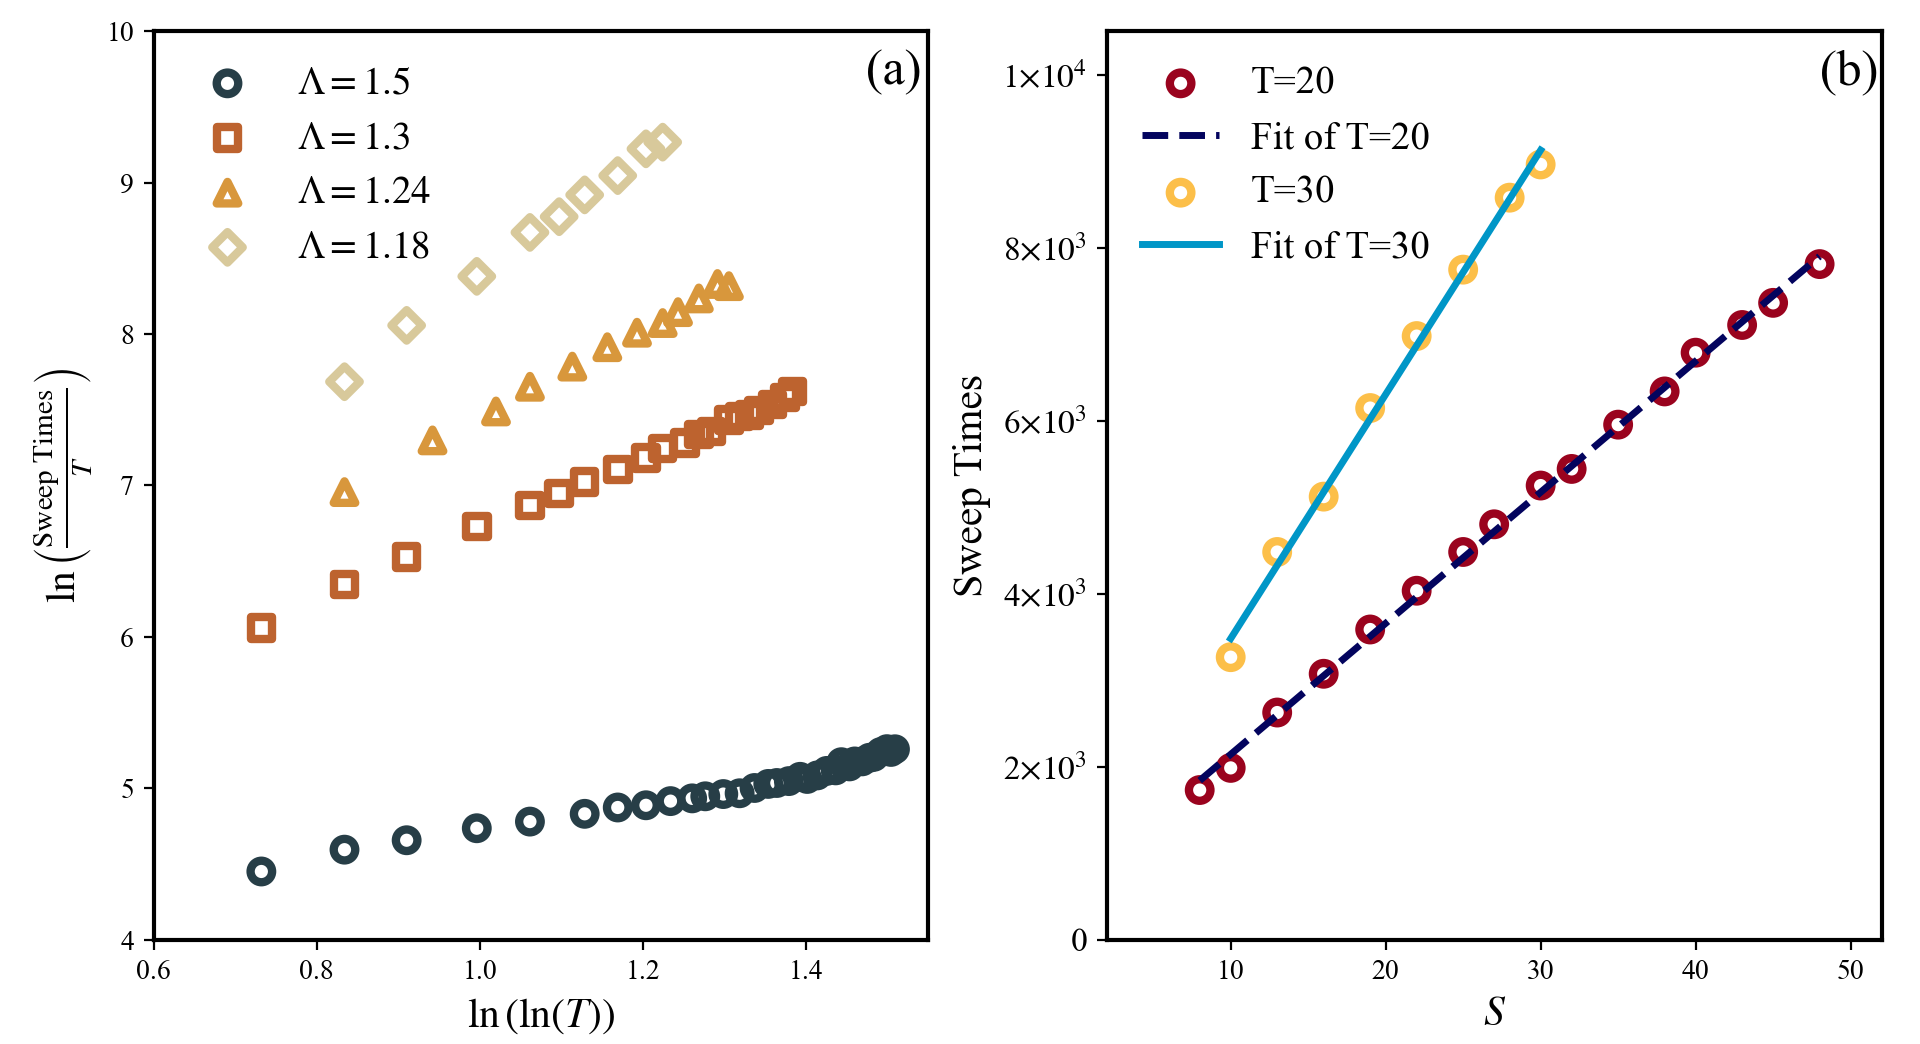
\includegraphics[width=\columnwidth,keepaspectratio]{../notes/images/MainNumericalResult.png}
    \caption{Numerical Result\jinguo{images should use the pdf format, the font size should be larger. Is it possible to verify that the Ising model is similar to the toy model? What is $T$ in the xlabel?}}
    \label{fig:main-numerical-result}
\end{figure}

\jinguo{you need to explain the results... what can we learn from the results?}
\jinguo{bad variable name: Sweep Time}
\Cref{fig:main-numerical-result} (a) shows the relationship between
$\ln(\ln(D))$ and $\ln(\frac{\text{Sweep Time}}{D})$ shoule be linear, which implies 
the time complexity along the ``Time'' direction should scale as $D\ln(D)^{f(\Lambda)}$. 
We then fit the slopes of each line and $\frac{1}{\ln(\Lambda)}$ and find the 
empirical constant $c$ in (\ref{eq:total-annealing-time}) to be $3$. [Fig. \ref{fig:main-numerical-result}(b)] shows 
the the relationship between Sweep Time and $S$ should be linear. Combining these two results, 
we can conclude that the time complexity should scales as $DS\log(D)^{1+\frac{1}{3\ln(\Lambda)}}$, 
which is consistent with our theoretical prediction in (\ref{eq:total-annealing-time}).

\jinguo{I hope we can also present some results for the random fluctuation model.
We just need some quantitative result about how the computing time scales with the depth.
}

% \begin{figure}[h]
%     \centering
%     \begin{minipage}[b]{0.485\columnwidth}
%         \centering
%         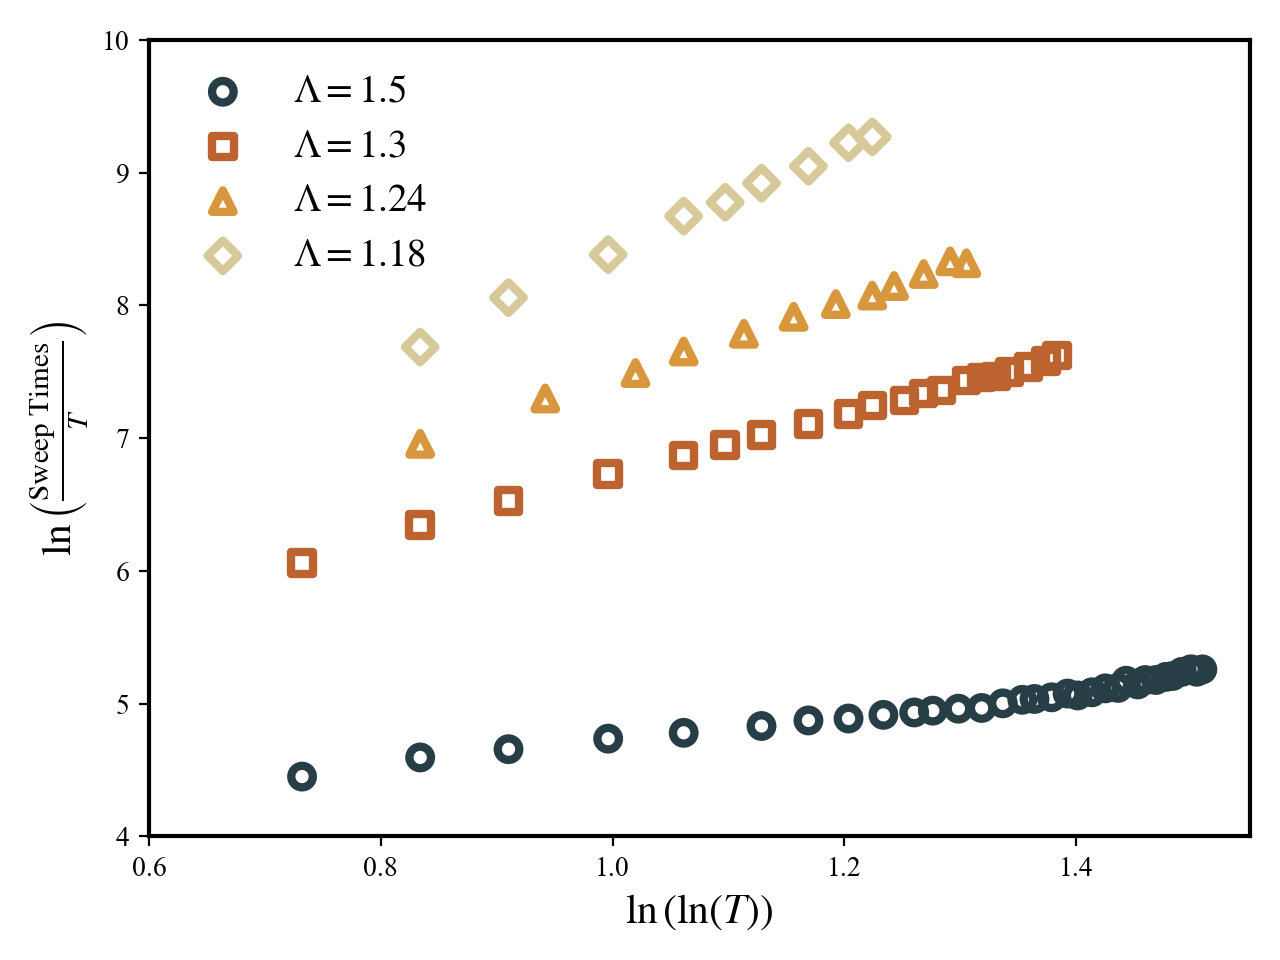
\includegraphics[width=\columnwidth,keepaspectratio]{../notes/images/TimeComplexityalongTaxis.png}
%         \caption{Time v.s. Depth of the material}
%         \label{fig:image1}
%     \end{minipage}
%     \hspace{0.001\columnwidth} % 两张图片之间的水平间距
%     \begin{minipage}[b]{0.485\columnwidth}
%         \centering
%         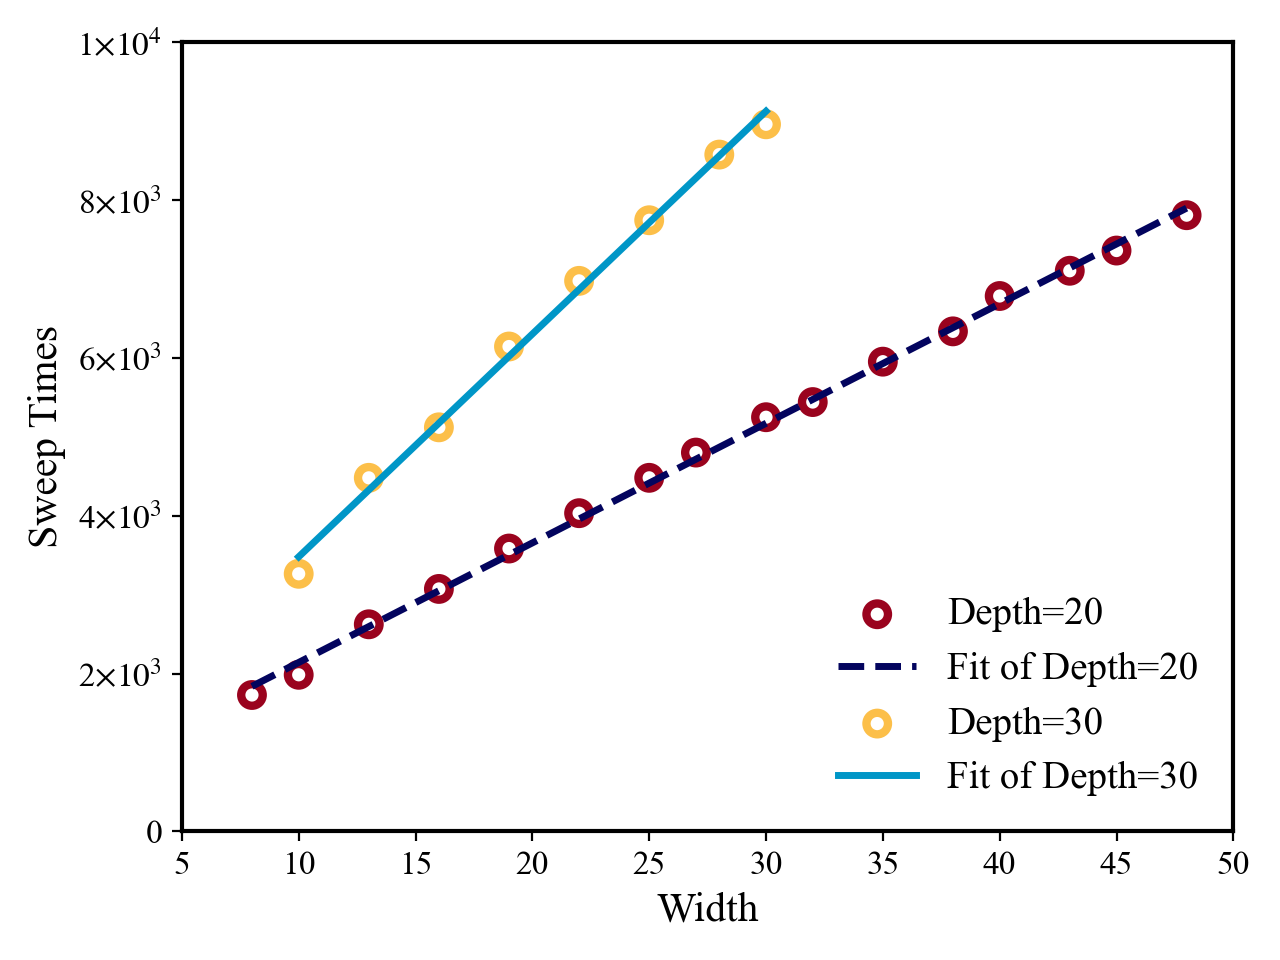
\includegraphics[width=\columnwidth,keepaspectratio]{../notes/images/toymodel_time_vs_width.png}
%         \caption{Time v.s. width of the material}
%         \label{fig:image2}
%     \end{minipage}
% \end{figure}

\section{Physical implementation on Ising machine}\label{spin-glass}

To examine whether this model could achieve a better performance when
using adiabatic methods, we need to generalize this energy function to
some good hamiltonian. There has already been work on mapping
combinatorial optimization problems to a spin-glass model (known as the
Ising Machine) and leveraging the properties of digital devices that
simulate this Ising Machine to find an appropriate ground state, which
encodes computational information~\cite{Aadit2022,Bybee2023}.



\section{Discussion and Outlook}
Connect real-world thermalization time and the simulated annealing time to explore the connection between time and energy cost per computation.
The emergence of wisdom?

Potential advantages: energy saving, parallelism, no size limits (robust to quantum effects). Disadvantages: slow, error-prone.

\begin{acknowledgments}
    %We thank Lei Wang, Madelyn Cain and XXX for helpful discussions on the simulation methods.
\end{acknowledgments}

%\bibliographystyle{apsrev4-1}
\bibliography{refs.bib}

\appendix

\section{Ising machine gadget design}\label{sec:gadget-design}
To map our toy model in \Cref{eq:toy-hamiltonian} to
spin-glass model, we used Linear Programming algorithm.
Linear problems are problems that can be express in standard form as

\begin{equation}
    \begin{split}
        &\min_{x \in \mathbb{R}^n} \sum_{i=1}^n c_ix_i\\
        &\text{s.t. } l_j \leq \sum_{i=1}^n a_{i,j}x_i \leq u_j, \; j=1,\ldots,m\\
        &p_i \leq x_i \leq q_i, \; i=1,\ldots, n
    \end{split}
\end{equation}

Here with a spin-glass consists $N$ atoms, we choose $n$ to be $\frac{N(N-1)}{2} + N$, which means each variable $x_i$ represents a correspond interaction energy $J_{u, v}$ or a correspond onsite energy $h_u$, we assigned aliases to these $x_i$ as $x_{u,v}$ or $x_{u}$.

Let the configuration space of the system be $S = \{\mathbf s_i\mid i=1,\ldots, 2^N\}$, each associated with an energy $H(\mathbf s_i)$. We denote the target states with minimum energy as $S_{\text{min}} \subseteq S$. We can express the linear programming problem as

\begin{equation}
    \begin{split}
        &\min_{J \in \mathbb{R}^{N(N{-}1)/2}, h\in \mathbb{R}^N} 0\\
        &H(\mathbf s_i) < H(\mathbf s_j), \forall \mathbf s_i \in S_{\text{min}}, \mathbf s_j \in S \setminus S_{\text{min}}\\
        &H(\mathbf s_i) = H(\mathbf s_j), \forall \mathbf s_i, \mathbf s_j \in S_{\text{min}}
    \end{split}
\end{equation}

Note that $H$ is a linear function of $J$ and $h$, so the
constraints are linear. The less constraints and equality constraints
can be easily transformed into inequality constraints by adding ancilla
variables.

We set the $S_{\text{min}}$ to be the eight degenerate ground states of the spin-glass model to implement the $110$ rule.
This is overly strict, as we do not consider the case that the ground states for different input signals to have degeneracy.
The minimum number of atoms required to satisfy the
constraints is 5. We set the target states to

\begin{table}[H]
    \centering
\begin{tabular}{|c|c|c|c|c|}
\hline
input 1 & input 2 & input 3 & output & ancilla \\
\hline
$\downarrow$ & $\downarrow$ & $\downarrow$ & $\downarrow$ & $?$ \\
$\downarrow$ & $\downarrow$ & $\uparrow$ & $\uparrow$ & $?$ \\
$\downarrow$ & $\uparrow$ & $\downarrow$ & $\uparrow$ & $?$ \\
$\downarrow$ & $\uparrow$ & $\uparrow$ & $\uparrow$ & $?$ \\
$\uparrow$ & $\downarrow$ & $\downarrow$ & $\downarrow$ & $?$ \\
$\uparrow$ & $\downarrow$ & $\uparrow$ & $\uparrow$ & $?$ \\
$\uparrow$ & $\uparrow$ & $\downarrow$ & $\uparrow$ & $?$ \\
$\uparrow$ & $\uparrow$ & $\uparrow$ & $\downarrow$ & $?$ \\
\hline
\end{tabular}
\caption{The eight degenerate ground states of the spin-glass model to implement the $110$ rule.}
\end{table}

where the ancilla bit in each row can be either $\uparrow$ or
$\downarrow$ (256 total possibilities). One of the solutions
satisfying the constraints is

\begin{equation}
J = \begin{pmatrix}
~\cdot~ & ~1~ & ~1~ & ~2~ & ~3~\\
\cdot & \cdot & 2 & 2 & 5\\
\cdot & \cdot & \cdot & 2 & 5\\
\cdot & \cdot & \cdot & \cdot & 6\\
\cdot & \cdot & \cdot & \cdot & \cdot
\end{pmatrix}, h = \begin{pmatrix}
~1~\\
2\\
2\\
2\\
5
\end{pmatrix}
\end{equation}

\section{Proof of the applicability of non-equilibrium SA}\label{proof-of_non-equilibrium-SA}

Assume there is another model where the temperature at the region with 
time coordinate $x$ at step $t$ is $T(x, t) = T_0\Lambda^{x - \eta t}$, where 
$\eta$ is cooling constant and $T_0$ satisfies $\exp(\frac{\Delta E_{max}}{T_0})\approx 1$, 
which means all the system stays in a relative high temperature initially. 
We called this model as temperature gradient model.

The cooling process starts at $t=0$ and ends at $t=t_{end}$, where $t_{end}$ satisfies
$\exp(\frac{\Delta E_{max}}{T_0\Lambda^{T - \eta t_{end}}}) \gg 1$, representing there wouldn't be any heat
fluctuations in the system. By noticing that we can define the effective heat zone
similarly to the moving heat bath model and then evaluating the time complexity, one can show that these two model are
equivalent.

The temperature gradient model can then be easily transform to
the energy gradient model in which equilibrilium SA can be applied by rescale local interacting and onsite energy.
The markov process can be treated with uniform temperature while rescale the energy associated with spin with Time-coordinate $x$
to be $E_{energy-gradient}(x) = E_{temp-gradient}(x)\Lambda^{-x}$. The acceptance probability is
invariant under this transformation.

\begin{equation}
    \exp\left({\frac{\Delta E_x}{T\Lambda^{x-\eta t}}}\right) = \exp\left({\frac{\Delta E_x\Lambda^{-x}}{T\Lambda^{-\eta t}}}\right) = \exp\left({\frac{\Delta E_x \Lambda^{-x}}{T(t)}}\right)
\end{equation}

We conducted numerical experiments to verify this equivalence under the condition
that $\Lambda = 1.3$ and $n=15$. The result is shown in [Fig. \ref{EGvsMHB}].
\begin{figure}[h]
    \centering
    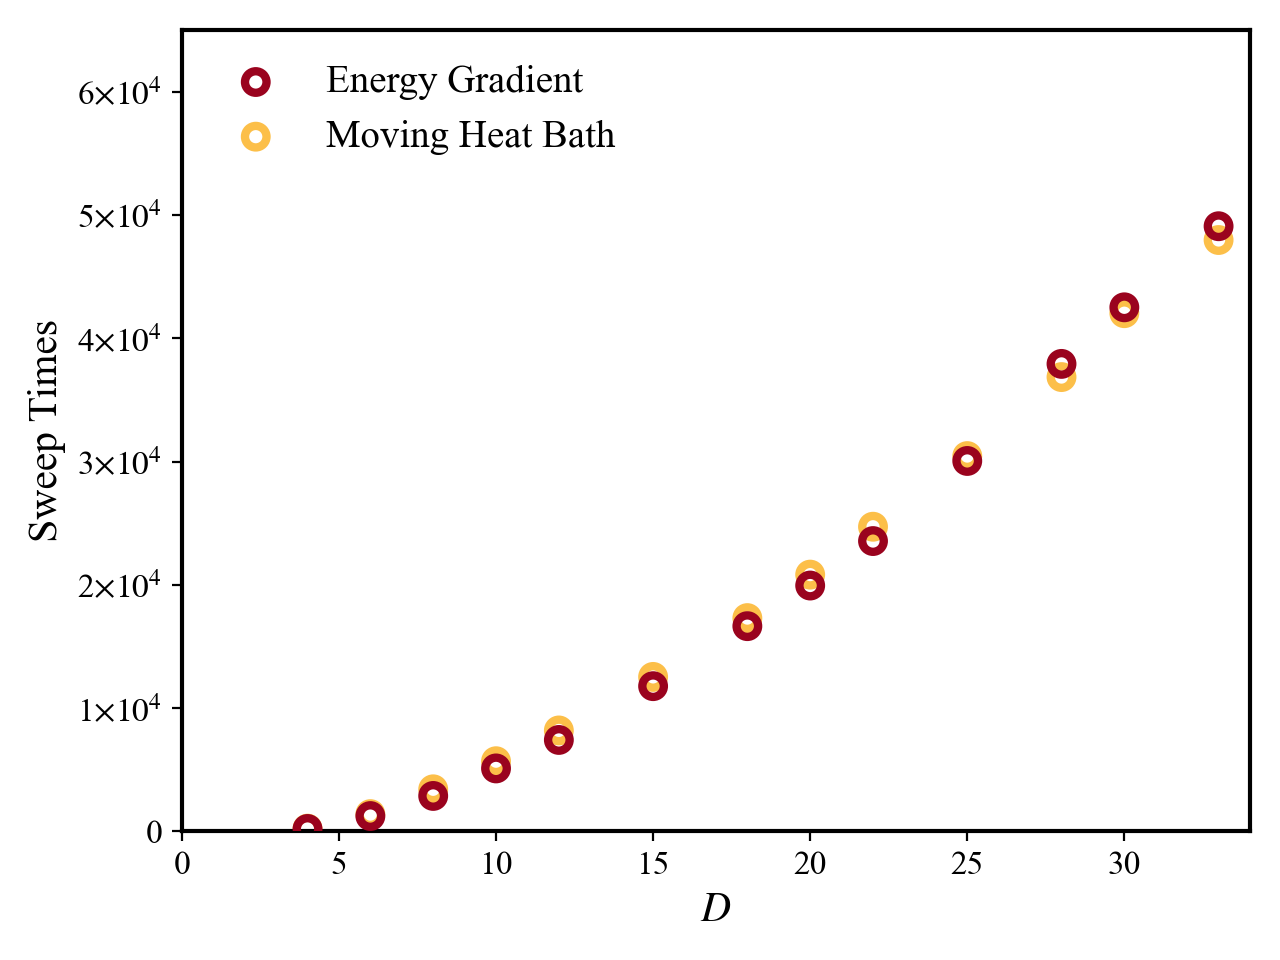
\includegraphics[width=\columnwidth,keepaspectratio]{../notes/images/EGvsMHB.png}
    \caption{Running time v.s Depth of the material}
    \label{EGvsMHB}
\end{figure}

\subsection{Speed and work}\label{speed-and-work}

The trade-off between the energy consumption and the speed of
computation~\cite{Feynman2018}. To avoid confusion, we emphasize the
``energy consumption'' is defined as the work done in a computational
process, which is the same as the amount of heat dissipated to the
environment. This quantity has a lower bound given by the Landauer
principle, which states that the work done in a computation is at least
$kT\ln 2$ per bit erased\cite{Reeb2014}.

Information erasure in the surface programmable material is proportional
to the volume of the material, which is $O(tS)$, where $t$ is the
time of computation, and $S$ is memory (proportional to the surface
area) of the material.

From the chemical reaction perspective, the speed of computation is
determined by the parameter $\lambda$.

\subsubsection{Quantum adiabatic annealing energy gap}\label{quantum-adiabatic-annealing-energy-gap}

One possible way is to use quantum adiabatic annealing: start from a
simple hamiltonian $H(0)$ and its simple ground state
$|\psi(0)\rangle$, then gradually change the parameters until reaching
the desire hamiltonian $H(t)$.

More specifically, set $\Delta(t=0) <0$ and $\Omega(t=0) =0$
initially, then first turning on $\Omega(t)$ to a non-zero value,
sweeping $\Delta(t)$ to final value, and finally turning off
$\Omega(t)$.

\begin{equation}
H_{QAA}(t) = \sum_{v\in V} (-\Delta(t)w_v \hat n_v + \Omega(t)\sigma_{v}^x) + \sum_{(u,w) \in E} U\hat n_u \hat n_w
\end{equation}

If the time evolution is sufficiently slow, then by the adiabatic
theorem, the system follows the instantaneous ground state, ending up in
the solution to the MWIS problem~\cite{Pichler2018}.
Then we only need to evalute
the minimum energy gap $\Delta_{QAA}$ between the ground and
first-excited states of instantaneous hamiltonian.

We set $\Omega = 1 \times 2\pi$ and sweep the $\Delta$ from $3
\times 2\pi$ to $40 \times 2\pi$ with 1*1 gadget. For deterministic
direction, we simply set the weight of the input vertices to $50$; as
for non-deterministic direction, we set the weight of the output vertice
to $50$.

Result listed as follows. \textbf{However, we didn't see cooling from
deterministic direction would give a smaller energy gap than the other
direction. We think that's because the size of this gadget is too
small.}

\begin{figure}
\centering
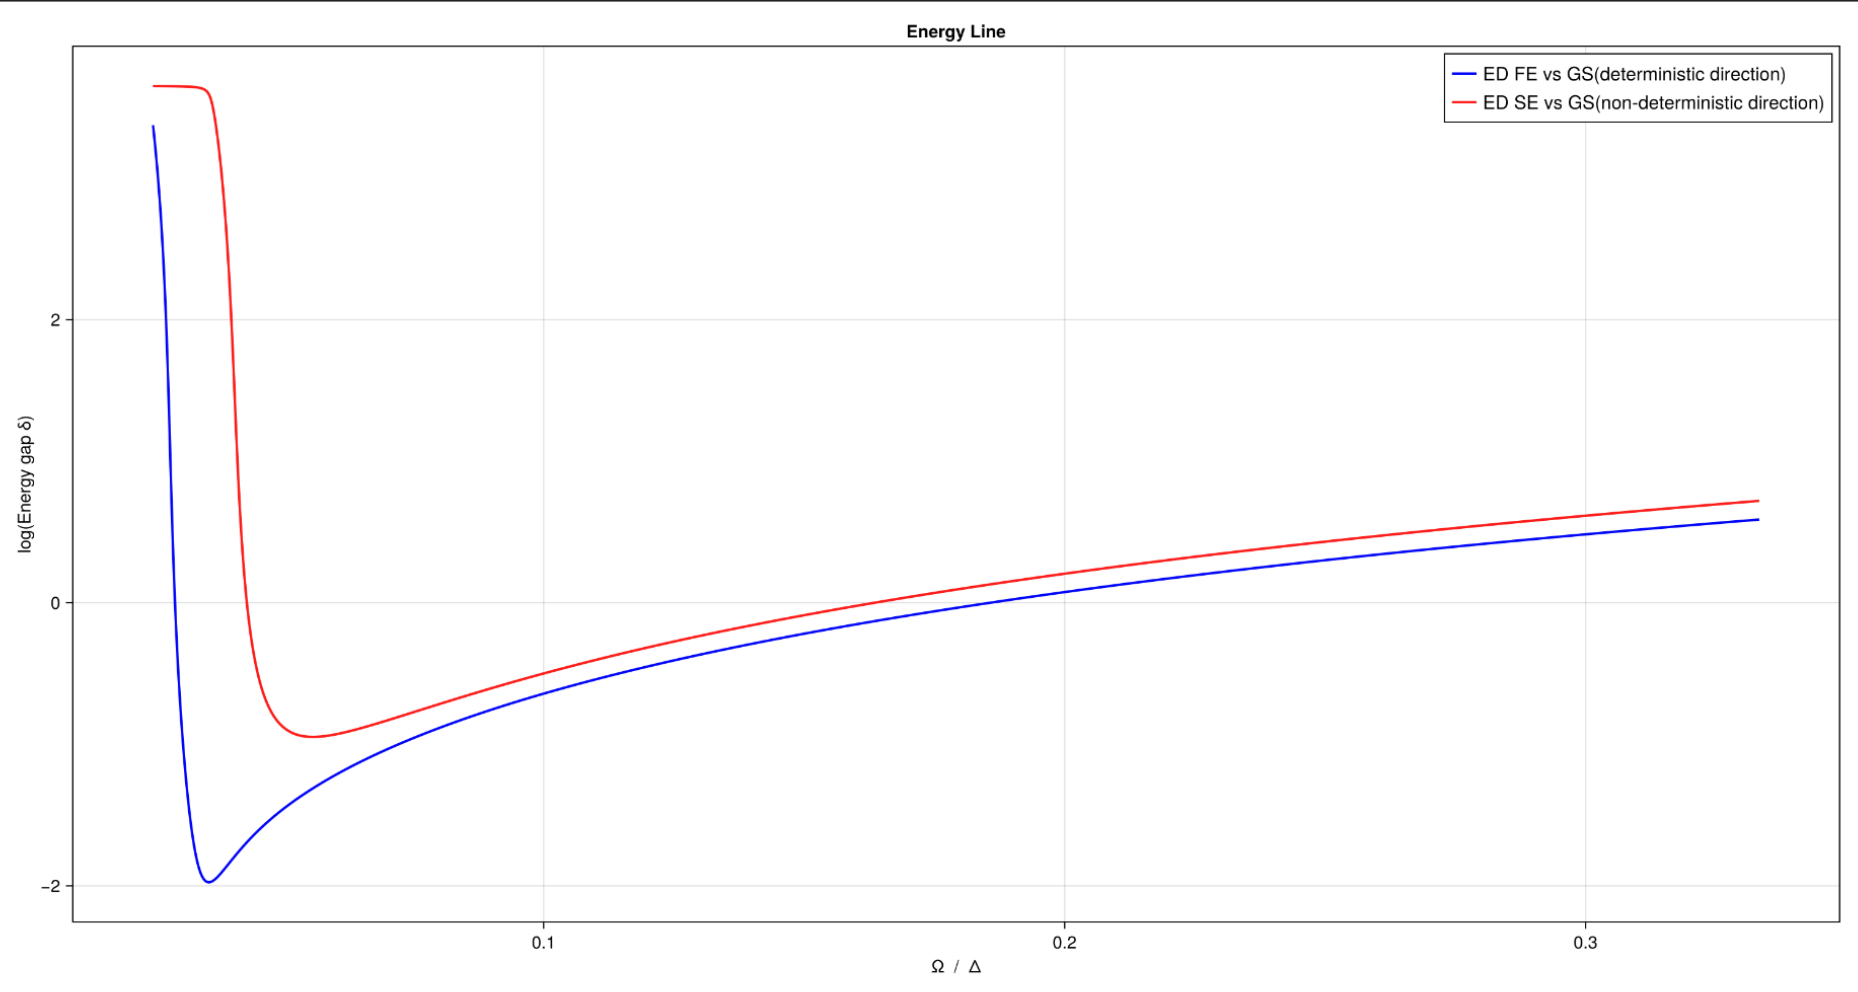
\includegraphics[width=\columnwidth]{../notes/images/energy_gap_1_gadget.png}
\caption{Alt text}
\end{figure}

\section{Classical Dynamics}\label{classical-dynamics-1}
We firstly tried classical adiabatic annealing with the classical-spin
mapping method~\cite{Wang2013}
\begin{equation}
\frac{\partial \vec M_i}{\partial t} = \vec M_{i} \times \vec H_{i}(t)
\end{equation}

where

\begin{equation}
\vec H_i(t) = -\frac{\partial H(t)}{\partial \vec M_i} 
\end{equation}

Here the hamiltonian of the system is

\begin{equation}
H(t) = \frac{t}{T}(\sum_{u,v}J_{u,v} M_{u,z}M_{v,z} + \sum_{u} h_u M_{u, z}) + (1-\frac{t}{T})(I\sum_{u}M_{u,x})
\end{equation}

The former term is the generally increasing target hamiltonian, the
latter term is a generally decreasing known Ising-transverse field. We
can explicitly write out the effective magnetic field.

\[
\vec H_{i}(t) = -\frac{t}{T}(\sum_{v}J_{i, v}M_{v,z} + h_i)\hat e_z - (1-\frac{t}{T})I\hat e_x
\]

Integrate the ordinary differential equation then we get the classical
dynamics of this spin-glass model. However, result shows that it is
extremely hard to find the solution when the number of layers exceed
$4$ (input layer is pinned).

The reason maybe that the mapped spin-glass model lies in the hard
region in ~\cite{Wang2013}. Because every interaction energy is positive, which
gives rise to strong frustration. Results in this reference also shows that even in
random spin-glass model, there exist hard instance that can't be solve.



\end{document}
